\documentclass[twoside]{book}

% Packages required by doxygen
\usepackage{calc}
\usepackage{doxygen}
\usepackage{graphicx}
\usepackage[utf8]{inputenc}
\usepackage{makeidx}
\usepackage{multicol}
\usepackage{multirow}
\usepackage{textcomp}
\usepackage[table]{xcolor}

% Font selection
\usepackage[T1]{fontenc}
\usepackage{mathptmx}
\usepackage[scaled=.90]{helvet}
\usepackage{courier}
\usepackage{amssymb}
\usepackage{sectsty}
\renewcommand{\familydefault}{\sfdefault}
\allsectionsfont{%
  \fontseries{bc}\selectfont%
  \color{darkgray}%
}
\renewcommand{\DoxyLabelFont}{%
  \fontseries{bc}\selectfont%
  \color{darkgray}%
}

% Page & text layout
\usepackage{geometry}
\geometry{%
  a4paper,%
  top=2.5cm,%
  bottom=2.5cm,%
  left=2.5cm,%
  right=2.5cm%
}
\tolerance=750
\hfuzz=15pt
\hbadness=750
\setlength{\emergencystretch}{15pt}
\setlength{\parindent}{0cm}
\setlength{\parskip}{0.2cm}
\makeatletter
\renewcommand{\paragraph}{%
  \@startsection{paragraph}{4}{0ex}{-1.0ex}{1.0ex}{%
    \normalfont\normalsize\bfseries\SS@parafont%
  }%
}
\renewcommand{\subparagraph}{%
  \@startsection{subparagraph}{5}{0ex}{-1.0ex}{1.0ex}{%
    \normalfont\normalsize\bfseries\SS@subparafont%
  }%
}
\makeatother

% Headers & footers
\usepackage{fancyhdr}
\pagestyle{fancyplain}
\fancyhead[LE]{\fancyplain{}{\bfseries\thepage}}
\fancyhead[CE]{\fancyplain{}{}}
\fancyhead[RE]{\fancyplain{}{\bfseries\leftmark}}
\fancyhead[LO]{\fancyplain{}{\bfseries\rightmark}}
\fancyhead[CO]{\fancyplain{}{}}
\fancyhead[RO]{\fancyplain{}{\bfseries\thepage}}
\fancyfoot[LE]{\fancyplain{}{}}
\fancyfoot[CE]{\fancyplain{}{}}
\fancyfoot[RE]{\fancyplain{}{\bfseries\scriptsize Generated on Thu May 6 2021 18\-:02\-:48 for My Project by Doxygen }}
\fancyfoot[LO]{\fancyplain{}{\bfseries\scriptsize Generated on Thu May 6 2021 18\-:02\-:48 for My Project by Doxygen }}
\fancyfoot[CO]{\fancyplain{}{}}
\fancyfoot[RO]{\fancyplain{}{}}
\renewcommand{\footrulewidth}{0.4pt}
\renewcommand{\chaptermark}[1]{%
  \markboth{#1}{}%
}
\renewcommand{\sectionmark}[1]{%
  \markright{\thesection\ #1}%
}

% Indices & bibliography
\usepackage{natbib}
\usepackage[titles]{tocloft}
\setcounter{tocdepth}{3}
\setcounter{secnumdepth}{5}
\makeindex

% Hyperlinks (required, but should be loaded last)
\usepackage{ifpdf}
\ifpdf
  \usepackage[pdftex,pagebackref=true]{hyperref}
\else
  \usepackage[ps2pdf,pagebackref=true]{hyperref}
\fi
\hypersetup{%
  colorlinks=true,%
  linkcolor=blue,%
  citecolor=blue,%
  unicode%
}

% Custom commands
\newcommand{\clearemptydoublepage}{%
  \newpage{\pagestyle{empty}\cleardoublepage}%
}


%===== C O N T E N T S =====

\begin{document}

% Titlepage & ToC
\hypersetup{pageanchor=false}
\pagenumbering{roman}
\begin{titlepage}
\vspace*{7cm}
\begin{center}%
{\Large My Project }\\
\vspace*{1cm}
{\large Generated by Doxygen 1.8.5}\\
\vspace*{0.5cm}
{\small Thu May 6 2021 18:02:48}\\
\end{center}
\end{titlepage}
\clearemptydoublepage
\tableofcontents
\clearemptydoublepage
\pagenumbering{arabic}
\hypersetup{pageanchor=true}

%--- Begin generated contents ---
\chapter{Distributed Point-\/\-To-\/\-Point Communication System}
\label{index}\hypertarget{index}{}\hypertarget{index_proj_desc}{}\section{Project Description}\label{index_proj_desc}
This program allows clients launched from any of 3 machines (acad, mcgonagall, \& csc552) to manipulate the records of a binary-\/encoded dataset stored on the server through the transmission of message packets over a T\-C\-P socket connection. \hypertarget{index_server_desc}{}\section{Server-\/side Description}\label{index_server_desc}
The server accepts incoming client connections, incrementing the number of clients and creating a new process for handling communications for each client. The server contains access to two separate files\-: The binary data file containing data records and a log file that documents all server operations. The server listens for incoming message packets on the socket, performing the corresponding operation for the received command. The server utilizes semaphores to ensure mutual exclusion amongst processes when reading and writing to/from both the dataset and the log file. The server operation is subsequently logged in the log file. \hypertarget{index_client_desc}{}\section{Client-\/side Description}\label{index_client_desc}
On startup, the client will allocate shared memory space and semaphores for all clients, if it is the first client on that machine to run. All subsequent clients on said machine will utilize the existing structures. It will then increment the number of clients in the shared memory space and subsequently find the next available block in the shared memory space, initializing its P\-I\-D and start\-Time fields. The client will utilize semaphores to ensure mutual exclusion amongst processes when reading/writing to the shared memory space and/or the log file. The client is presented with a menu of commands that can be issued to the server and subsequently prompted for their selection. The client will then be prompted for any other necessary information relevant to the command and send it over the socket to the server. All Client operations are then logged in the client log file. The client may perform as many operations as they wish until they specify to exit. \hypertarget{index_readWrite}{}\section{Readers-\/\-Writers Problem}\label{index_readWrite}
The server will utilize a strong writers' preference that allows concurrent reader access for accessing the binary data file. The client will utilize a strong writers' preference that allows concurrent reader access for accessing shared memory. Both the client and the server will utilize a weak reader's preference with concurrent reader access for accessing their log files. \hypertarget{index_menu}{}\section{Menu Options\-:}\label{index_menu}
\hypertarget{index_new_record}{}\subsection{New Record}\label{index_new_record}
Upon selecting the New Record menu option, the client will prompt the user for all necessary fields for a record and validate the user's input. The client will then issue the N\-E\-W command to the server, indicating a new record is to be added, passing it the newly defined record, and awaiting the server's acknowledgment message. \hypertarget{index_display_record}{}\subsection{Display Record}\label{index_display_record}
Upon selecting the Display Record menu option, the client will issue the C\-N\-T command to the server, indicating a request for the number of records, and await the server's response. Upon receiving the number of records, the client will prompt the user for the index of a record between 1 and the received number of records to be displayed, validating the entered value is in that range. The user also has the option to enter -\/999 to display all records. The client will then issue the G\-E\-T command, indicating a request for a particular record or set of records, and await the server's response. The client will then display the received record(s) to the user. \hypertarget{index_change_record}{}\subsection{Change Record}\label{index_change_record}
Upon selecting the Change Record menu option, the client will perform the same operations as Display Record, however, without the option to display all records. After the selected record is displayed, the client will prompt the user to select a field to edit from a menu of editable fields and then prompt the user for a value for that field, reprompting for invalid input if necessary. The client will then issue the F\-I\-X command to the server, indicating a record is to be updated, passing it the newly updated record and its index, and await the server's acknowledgment message. \hypertarget{index_show_log}{}\subsection{Show Server Log}\label{index_show_log}
Upon selecting the Show Log menu option, the client will issue the L\-O\-G command to the server, indicating a request for the contents of the log and await the server's response. The client will receive the number of log records to expect, followed by a stream of individual log records. The client will print each log record to the user as it is received. \hypertarget{index_view_log}{}\subsection{View Client Log}\label{index_view_log}
Upon selecting the View Client Log menu option, the client will access and print the contents of its machine's log file one record a time until it reaches the end of the file. \hypertarget{index_list_clients}{}\subsection{List Local Clients}\label{index_list_clients}
Upon selecting the List Local Clients menu option, the client will access the shared memory and retrieve each of the local client's process I\-Ds one at a time, displaying them to the user 
\chapter{Hierarchical Index}
\section{Class Hierarchy}
This inheritance list is sorted roughly, but not completely, alphabetically\-:\begin{DoxyCompactList}
\item \contentsline{section}{Data\-Record}{\pageref{classDataRecord}}{}
\item \contentsline{section}{Log\-Bin\-R\-W\-Sem\-Monitor}{\pageref{classLogBinRWSemMonitor}}{}
\item \contentsline{section}{msg\-Packet}{\pageref{structmsgPacket}}{}
\begin{DoxyCompactList}
\item \contentsline{section}{int\-Msg\-Packet}{\pageref{structintMsgPacket}}{}
\item \contentsline{section}{int\-Rec\-Msg\-Packet}{\pageref{structintRecMsgPacket}}{}
\begin{DoxyCompactList}
\item \contentsline{section}{ser\-Msg\-Packet}{\pageref{structserMsgPacket}}{}
\end{DoxyCompactList}
\item \contentsline{section}{log\-Msg\-Packet}{\pageref{structlogMsgPacket}}{}
\item \contentsline{section}{rec\-Msg\-Packet}{\pageref{structrecMsgPacket}}{}
\end{DoxyCompactList}
\item \contentsline{section}{Semaphore\-Set}{\pageref{classSemaphoreSet}}{}
\item \contentsline{section}{Shared\-Memory\-Manager\-:\-:shared\-Mem\-Block}{\pageref{structSharedMemoryManager_1_1sharedMemBlock}}{}
\item \contentsline{section}{Shared\-Memory\-Manager}{\pageref{classSharedMemoryManager}}{}
\item \contentsline{section}{string\-To\-Month\-Converter}{\pageref{classstringToMonthConverter}}{}
\end{DoxyCompactList}

\chapter{Class Index}
\section{Class List}
Here are the classes, structs, unions and interfaces with brief descriptions\-:\begin{DoxyCompactList}
\item\contentsline{section}{\hyperlink{classDataRecord}{Data\-Record} \\*Class for holding a single record of Data }{\pageref{classDataRecord}}{}
\item\contentsline{section}{\hyperlink{structintMsgPacket}{int\-Msg\-Packet} \\*Sub-\/\-Struct T\-C\-P message packet for transmitting record count \& indexes }{\pageref{structintMsgPacket}}{}
\item\contentsline{section}{\hyperlink{structintRecMsgPacket}{int\-Rec\-Msg\-Packet} \\*Sub-\/\-Struct T\-C\-P message packet for transmitting a record and its index }{\pageref{structintRecMsgPacket}}{}
\item\contentsline{section}{\hyperlink{classLogBinRWSemMonitor}{Log\-Bin\-R\-W\-Sem\-Monitor} \\*Monitor for managing Readers and Writers to the bin and log files using semaphores }{\pageref{classLogBinRWSemMonitor}}{}
\item\contentsline{section}{\hyperlink{structlogMsgPacket}{log\-Msg\-Packet} \\*Sub-\/\-Struct T\-C\-P message packet for transmitting log records }{\pageref{structlogMsgPacket}}{}
\item\contentsline{section}{\hyperlink{structmsgPacket}{msg\-Packet} \\*Base Struct T\-C\-P message packet }{\pageref{structmsgPacket}}{}
\item\contentsline{section}{\hyperlink{structrecMsgPacket}{rec\-Msg\-Packet} \\*Sub-\/\-Struct T\-C\-P message packet for transmitting records }{\pageref{structrecMsgPacket}}{}
\item\contentsline{section}{\hyperlink{classSemaphoreSet}{Semaphore\-Set} \\*Wrapper Class for U\-N\-I\-X System V Semaphores }{\pageref{classSemaphoreSet}}{}
\item\contentsline{section}{\hyperlink{structserMsgPacket}{ser\-Msg\-Packet} \\*Union Struct T\-C\-P message packet for receiving messages on server side }{\pageref{structserMsgPacket}}{}
\item\contentsline{section}{\hyperlink{structSharedMemoryManager_1_1sharedMemBlock}{Shared\-Memory\-Manager\-::shared\-Mem\-Block} \\*Container struct of all fields in a client process' shared memory block }{\pageref{structSharedMemoryManager_1_1sharedMemBlock}}{}
\item\contentsline{section}{\hyperlink{classSharedMemoryManager}{Shared\-Memory\-Manager} \\*Wrapper\-Class Implementation of U\-N\-I\-X Shared Memory for easier creation, storage, and retrieval }{\pageref{classSharedMemoryManager}}{}
\item\contentsline{section}{\hyperlink{classstringToMonthConverter}{string\-To\-Month\-Converter} \\*Used to map enum values to valid input strings for the month field of new records }{\pageref{classstringToMonthConverter}}{}
\end{DoxyCompactList}

\chapter{File Index}
\section{File List}
Here is a list of all documented files with brief descriptions\-:\begin{DoxyCompactList}
\item\contentsline{section}{\hyperlink{client_8cpp}{client.\-cpp} \\*Client side of the T\-C\-P Distributed Information System implementation C\-S\-C552 Dr. Spiegel Spring 2020 }{\pageref{client_8cpp}}{}
\item\contentsline{section}{\hyperlink{createBin_8cpp}{create\-Bin.\-cpp} \\*C\-S\-C552 Dr. Spiegel Spring 2020 Transfers data from an input .csv file into an output binary-\/encoded file, whose filenames are provided as command-\/line arguments. Returns the number of lines read from the in\-File or failed open flags }{\pageref{createBin_8cpp}}{}
\item\contentsline{section}{\hyperlink{DataRecord_8cpp}{Data\-Record.\-cpp} \\*A structure for storing, manipulating, and exporting records from the dataset }{\pageref{DataRecord_8cpp}}{}
\item\contentsline{section}{\hyperlink{LogBinRWSemMonitor_8cpp}{Log\-Bin\-R\-W\-Sem\-Monitor.\-cpp} \\*Implementation of a Monitors for the Readers-\/\-Writers problem using semaphores Uses strong writers preference while allowing concurrent reader access for the bin file and weak readers preference while allowing concurrent reader access for the log file }{\pageref{LogBinRWSemMonitor_8cpp}}{}
\item\contentsline{section}{\hyperlink{msgPackets_8cpp}{msg\-Packets.\-cpp} \\*Header file defining the various packets used to transmit data across the T\-C\-P socket connection. C\-S\-C552 Dr. Spiegel Spring 2020 }{\pageref{msgPackets_8cpp}}{}
\item\contentsline{section}{\hyperlink{SemaphoreSet_8cpp}{Semaphore\-Set.\-cpp} \\*Wrapper Class Implementation of U\-N\-I\-X System V semaphores }{\pageref{SemaphoreSet_8cpp}}{}
\item\contentsline{section}{\hyperlink{server_8cpp}{server.\-cpp} \\*Server side of the T\-C\-P Distributed Information System implementation C\-S\-C552 Dr. Spiegel Spring 2020 }{\pageref{server_8cpp}}{}
\item\contentsline{section}{\hyperlink{SharedMemoryManager_8cpp}{Shared\-Memory\-Manager.\-cpp} \\*Wrapper Class Implementation of System V Shared Memory for use with the Distributed Point-\/\-To-\/\-Point Communications System. It should be noted that the term shared memory space refers to the entire allocated address space shared between all client processes while the term shared memory block refers to a segment in the shared memory space containing a single client process' data. C\-S\-C552 Dr. Spiegel Spring 2020 }{\pageref{SharedMemoryManager_8cpp}}{}
\end{DoxyCompactList}

\chapter{Class Documentation}
\hypertarget{classDataRecord}{\section{Data\-Record Class Reference}
\label{classDataRecord}\index{Data\-Record@{Data\-Record}}
}


Class for holding a single record of Data.  


\subsection*{Public Member Functions}
\begin{DoxyCompactItemize}
\item 
\hypertarget{classDataRecord_ad93a5bf8b22613e9723e98251dad7912}{\hyperlink{classDataRecord_ad93a5bf8b22613e9723e98251dad7912}{Data\-Record} ()}\label{classDataRecord_ad93a5bf8b22613e9723e98251dad7912}

\begin{DoxyCompactList}\small\item\em Default Constructor for the \hyperlink{classDataRecord}{Data\-Record} object. \end{DoxyCompactList}\item 
\hyperlink{classDataRecord_a8e7efc362d0c64ca189f9ac2abd56e8e}{Data\-Record} (string month\-Year, float accessories, float hardware, float software, float total, int rec\-Idx=-\/1)
\begin{DoxyCompactList}\small\item\em Constructs a \hyperlink{classDataRecord}{Data\-Record} object using data field values. \end{DoxyCompactList}\item 
\hyperlink{classDataRecord_ae0b2d3655024922143f35a022d9d965b}{Data\-Record} (string record, int rec\-Idx=-\/1)
\begin{DoxyCompactList}\small\item\em Constructs a \hyperlink{classDataRecord}{Data\-Record} object given a record string read from the bin file, by parsing it into the object's data members. \end{DoxyCompactList}\item 
string \hyperlink{classDataRecord_a2f5721666868ded376f3edff99cfb1b9}{field\-To\-String} (float field)
\begin{DoxyCompactList}\small\item\em Converts fields of type float to their fixed precision string types. \end{DoxyCompactList}\item 
int \hyperlink{classDataRecord_a0f679d9af4ac1a0f1ad0017c08b88278}{get\-Record\-Index} ()
\begin{DoxyCompactList}\small\item\em Retrieves the idx data member. \end{DoxyCompactList}\item 
\hypertarget{classDataRecord_a601e4f559dfece4c61d2982bc01165b4}{void \hyperlink{classDataRecord_a601e4f559dfece4c61d2982bc01165b4}{print\-Record} ()}\label{classDataRecord_a601e4f559dfece4c61d2982bc01165b4}

\begin{DoxyCompactList}\small\item\em Prints the \hyperlink{classDataRecord}{Data\-Record} object in a well-\/formatted manner. \end{DoxyCompactList}\item 
void \hyperlink{classDataRecord_a17dd98967502f3fdbfd8d611e50b8cf1}{set\-Accessories} (float val)
\begin{DoxyCompactList}\small\item\em Sets the accessories data member to the provided value. \end{DoxyCompactList}\item 
void \hyperlink{classDataRecord_a11be3829611599f63d8cdc1b78f2e075}{set\-Hardware} (float val)
\begin{DoxyCompactList}\small\item\em Sets the hardware data member to the provided value. \end{DoxyCompactList}\item 
void \hyperlink{classDataRecord_a0bca4a4d9088733e0d83cc6f602a400a}{set\-Software} (float val)
\begin{DoxyCompactList}\small\item\em Sets the Software data member to the provided value. \end{DoxyCompactList}\item 
void \hyperlink{classDataRecord_a59a60fd621917ea907a8020d929d75ea}{set\-Total} (float val)
\begin{DoxyCompactList}\small\item\em Sets the total data member to the provided value. \end{DoxyCompactList}\item 
string \hyperlink{classDataRecord_a0c7343d8583d1c3c5582e683ff54daed}{to\-String} ()
\begin{DoxyCompactList}\small\item\em Converts the \hyperlink{classDataRecord}{Data\-Record} object to a string. \end{DoxyCompactList}\item 
\hypertarget{classDataRecord_ae5aece25155248b9cfb6750f84c4249f}{void \hyperlink{classDataRecord_ae5aece25155248b9cfb6750f84c4249f}{update\-Total} ()}\label{classDataRecord_ae5aece25155248b9cfb6750f84c4249f}

\begin{DoxyCompactList}\small\item\em Updates the total field by summing the hardware, software, and accessories fields. \end{DoxyCompactList}\end{DoxyCompactItemize}


\subsection{Detailed Description}
Class for holding a single record of Data. 

\subsection{Constructor \& Destructor Documentation}
\hypertarget{classDataRecord_a8e7efc362d0c64ca189f9ac2abd56e8e}{\index{Data\-Record@{Data\-Record}!Data\-Record@{Data\-Record}}
\index{Data\-Record@{Data\-Record}!DataRecord@{Data\-Record}}
\subsubsection[{Data\-Record}]{\setlength{\rightskip}{0pt plus 5cm}Data\-Record\-::\-Data\-Record (
\begin{DoxyParamCaption}
\item[{string}]{month\-Year, }
\item[{float}]{accessories, }
\item[{float}]{hardware, }
\item[{float}]{software, }
\item[{float}]{total, }
\item[{int}]{rec\-Idx = {\ttfamily -\/1}}
\end{DoxyParamCaption}
)\hspace{0.3cm}{\ttfamily [inline]}}}\label{classDataRecord_a8e7efc362d0c64ca189f9ac2abd56e8e}


Constructs a \hyperlink{classDataRecord}{Data\-Record} object using data field values. 


\begin{DoxyParams}{Parameters}
{\em month\-Year} & The month and year of captured revenue \\
\hline
{\em accessories} & The generated revenue from accessories \\
\hline
{\em hardware} & The generated revenue from hardware \\
\hline
{\em software} & The generated revenue from software \\
\hline
{\em total} & The total generated revenue \\
\hline
{\em rec\-Idx} & The index of the record, -\/1 by default \\
\hline
\end{DoxyParams}
\hypertarget{classDataRecord_ae0b2d3655024922143f35a022d9d965b}{\index{Data\-Record@{Data\-Record}!Data\-Record@{Data\-Record}}
\index{Data\-Record@{Data\-Record}!DataRecord@{Data\-Record}}
\subsubsection[{Data\-Record}]{\setlength{\rightskip}{0pt plus 5cm}Data\-Record\-::\-Data\-Record (
\begin{DoxyParamCaption}
\item[{string}]{record, }
\item[{int}]{rec\-Idx = {\ttfamily -\/1}}
\end{DoxyParamCaption}
)\hspace{0.3cm}{\ttfamily [inline]}}}\label{classDataRecord_ae0b2d3655024922143f35a022d9d965b}


Constructs a \hyperlink{classDataRecord}{Data\-Record} object given a record string read from the bin file, by parsing it into the object's data members. 


\begin{DoxyParams}{Parameters}
{\em record} & Record string read from the file. \\
\hline
{\em rec\-Idx} & Index of the \hyperlink{classDataRecord}{Data\-Record} in the server bin file \\
\hline
\end{DoxyParams}


\subsection{Member Function Documentation}
\hypertarget{classDataRecord_a2f5721666868ded376f3edff99cfb1b9}{\index{Data\-Record@{Data\-Record}!field\-To\-String@{field\-To\-String}}
\index{field\-To\-String@{field\-To\-String}!DataRecord@{Data\-Record}}
\subsubsection[{field\-To\-String}]{\setlength{\rightskip}{0pt plus 5cm}string Data\-Record\-::field\-To\-String (
\begin{DoxyParamCaption}
\item[{float}]{field}
\end{DoxyParamCaption}
)\hspace{0.3cm}{\ttfamily [inline]}}}\label{classDataRecord_a2f5721666868ded376f3edff99cfb1b9}


Converts fields of type float to their fixed precision string types. 


\begin{DoxyParams}{Parameters}
{\em field} & Float Data field \\
\hline
\end{DoxyParams}
\begin{DoxyReturn}{Returns}
A fixed precision float-\/converted string. 
\end{DoxyReturn}
\hypertarget{classDataRecord_a0f679d9af4ac1a0f1ad0017c08b88278}{\index{Data\-Record@{Data\-Record}!get\-Record\-Index@{get\-Record\-Index}}
\index{get\-Record\-Index@{get\-Record\-Index}!DataRecord@{Data\-Record}}
\subsubsection[{get\-Record\-Index}]{\setlength{\rightskip}{0pt plus 5cm}int Data\-Record\-::get\-Record\-Index (
\begin{DoxyParamCaption}
{}
\end{DoxyParamCaption}
)\hspace{0.3cm}{\ttfamily [inline]}}}\label{classDataRecord_a0f679d9af4ac1a0f1ad0017c08b88278}


Retrieves the idx data member. 

\begin{DoxyReturn}{Returns}
The value of the idx member 
\end{DoxyReturn}
\hypertarget{classDataRecord_a17dd98967502f3fdbfd8d611e50b8cf1}{\index{Data\-Record@{Data\-Record}!set\-Accessories@{set\-Accessories}}
\index{set\-Accessories@{set\-Accessories}!DataRecord@{Data\-Record}}
\subsubsection[{set\-Accessories}]{\setlength{\rightskip}{0pt plus 5cm}void Data\-Record\-::set\-Accessories (
\begin{DoxyParamCaption}
\item[{float}]{val}
\end{DoxyParamCaption}
)\hspace{0.3cm}{\ttfamily [inline]}}}\label{classDataRecord_a17dd98967502f3fdbfd8d611e50b8cf1}


Sets the accessories data member to the provided value. 


\begin{DoxyParams}{Parameters}
{\em val} & Value to set data member to \\
\hline
\end{DoxyParams}
\hypertarget{classDataRecord_a11be3829611599f63d8cdc1b78f2e075}{\index{Data\-Record@{Data\-Record}!set\-Hardware@{set\-Hardware}}
\index{set\-Hardware@{set\-Hardware}!DataRecord@{Data\-Record}}
\subsubsection[{set\-Hardware}]{\setlength{\rightskip}{0pt plus 5cm}void Data\-Record\-::set\-Hardware (
\begin{DoxyParamCaption}
\item[{float}]{val}
\end{DoxyParamCaption}
)\hspace{0.3cm}{\ttfamily [inline]}}}\label{classDataRecord_a11be3829611599f63d8cdc1b78f2e075}


Sets the hardware data member to the provided value. 


\begin{DoxyParams}{Parameters}
{\em val} & Value to set data member to \\
\hline
\end{DoxyParams}
\hypertarget{classDataRecord_a0bca4a4d9088733e0d83cc6f602a400a}{\index{Data\-Record@{Data\-Record}!set\-Software@{set\-Software}}
\index{set\-Software@{set\-Software}!DataRecord@{Data\-Record}}
\subsubsection[{set\-Software}]{\setlength{\rightskip}{0pt plus 5cm}void Data\-Record\-::set\-Software (
\begin{DoxyParamCaption}
\item[{float}]{val}
\end{DoxyParamCaption}
)\hspace{0.3cm}{\ttfamily [inline]}}}\label{classDataRecord_a0bca4a4d9088733e0d83cc6f602a400a}


Sets the Software data member to the provided value. 


\begin{DoxyParams}{Parameters}
{\em val} & Value to set data member to \\
\hline
\end{DoxyParams}
\hypertarget{classDataRecord_a59a60fd621917ea907a8020d929d75ea}{\index{Data\-Record@{Data\-Record}!set\-Total@{set\-Total}}
\index{set\-Total@{set\-Total}!DataRecord@{Data\-Record}}
\subsubsection[{set\-Total}]{\setlength{\rightskip}{0pt plus 5cm}void Data\-Record\-::set\-Total (
\begin{DoxyParamCaption}
\item[{float}]{val}
\end{DoxyParamCaption}
)\hspace{0.3cm}{\ttfamily [inline]}}}\label{classDataRecord_a59a60fd621917ea907a8020d929d75ea}


Sets the total data member to the provided value. 


\begin{DoxyParams}{Parameters}
{\em val} & Value to set data member to \\
\hline
\end{DoxyParams}
\hypertarget{classDataRecord_a0c7343d8583d1c3c5582e683ff54daed}{\index{Data\-Record@{Data\-Record}!to\-String@{to\-String}}
\index{to\-String@{to\-String}!DataRecord@{Data\-Record}}
\subsubsection[{to\-String}]{\setlength{\rightskip}{0pt plus 5cm}string Data\-Record\-::to\-String (
\begin{DoxyParamCaption}
{}
\end{DoxyParamCaption}
)\hspace{0.3cm}{\ttfamily [inline]}}}\label{classDataRecord_a0c7343d8583d1c3c5582e683ff54daed}


Converts the \hyperlink{classDataRecord}{Data\-Record} object to a string. 

\begin{DoxyReturn}{Returns}
The string representation of the \hyperlink{classDataRecord}{Data\-Record} object 
\end{DoxyReturn}


The documentation for this class was generated from the following file\-:\begin{DoxyCompactItemize}
\item 
\hyperlink{DataRecord_8cpp}{Data\-Record.\-cpp}\end{DoxyCompactItemize}

\input{structintMsgPacket}
\hypertarget{structintRecMsgPacket}{\section{int\-Rec\-Msg\-Packet Struct Reference}
\label{structintRecMsgPacket}\index{int\-Rec\-Msg\-Packet@{int\-Rec\-Msg\-Packet}}
}


Sub-\/\-Struct T\-C\-P message packet for transmitting a record and its index.  


Inheritance diagram for int\-Rec\-Msg\-Packet\-:\begin{figure}[H]
\begin{center}
\leavevmode
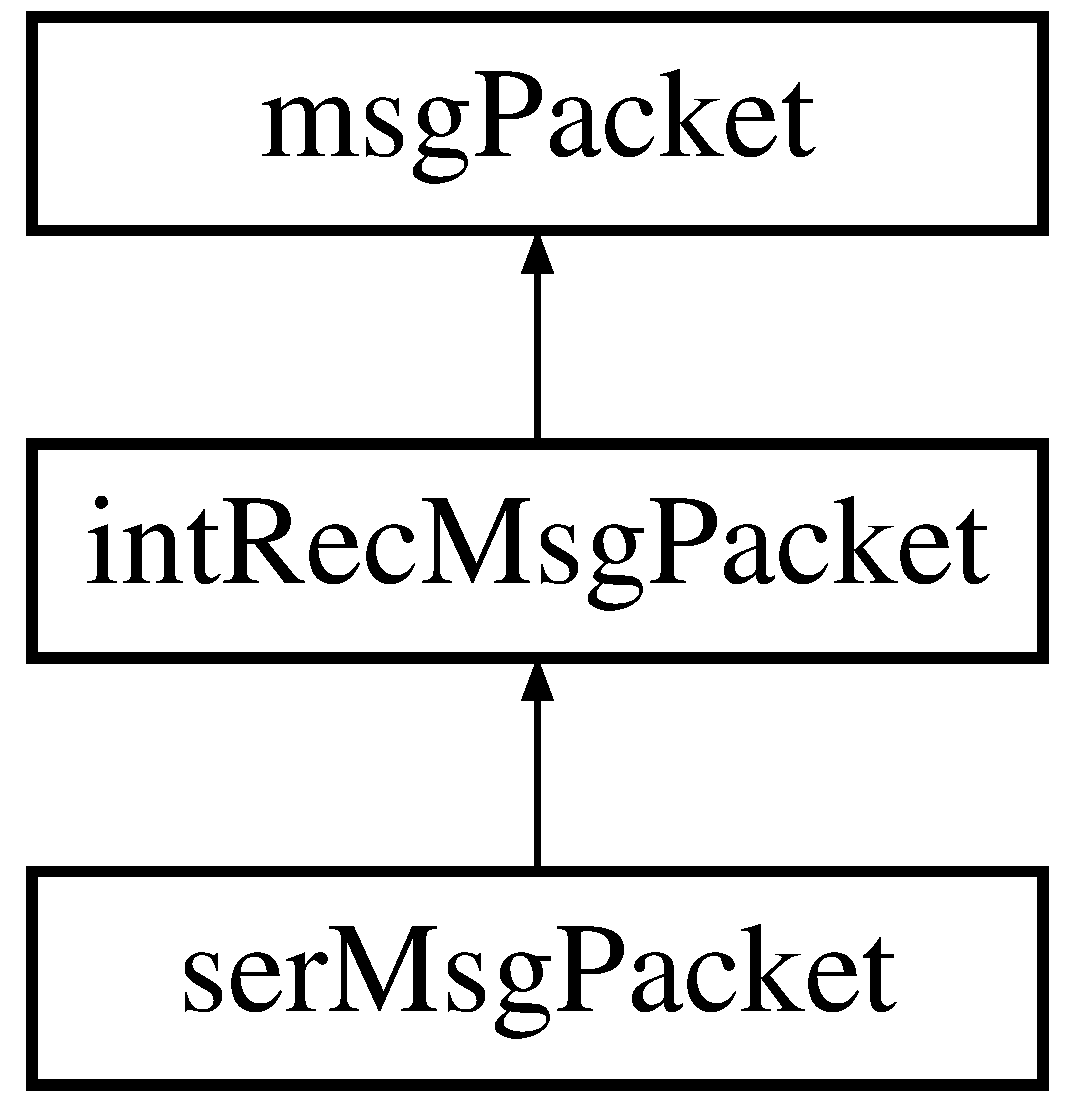
\includegraphics[height=3.000000cm]{structintRecMsgPacket}
\end{center}
\end{figure}
\subsection*{Public Member Functions}
\begin{DoxyCompactItemize}
\item 
\hypertarget{structintRecMsgPacket_a2f337aa26e3c8bf95404e3958f306c3b}{\hyperlink{structintRecMsgPacket_a2f337aa26e3c8bf95404e3958f306c3b}{int\-Rec\-Msg\-Packet} ()}\label{structintRecMsgPacket_a2f337aa26e3c8bf95404e3958f306c3b}

\begin{DoxyCompactList}\small\item\em Default constructor for \hyperlink{structintRecMsgPacket}{int\-Rec\-Msg\-Packet}. \end{DoxyCompactList}\item 
\hyperlink{structintRecMsgPacket_af0017da02a0021d5674c88bfb9151f1e}{int\-Rec\-Msg\-Packet} (pid\-\_\-t \hyperlink{structmsgPacket_a294c1f456116eb9177b31ab8b5577f86}{sender}, const char \hyperlink{structmsgPacket_a8b49c124b4ca2ed872692333b71d74fd}{cmd}\mbox{[}$\,$\mbox{]}, int \hyperlink{structintRecMsgPacket_a09009e50e4f452b7fea038fcb5f8e382}{val}, char \hyperlink{structintRecMsgPacket_a4edab3e169d3d5d2ceced40d663e8055}{record}\mbox{[}$\,$\mbox{]})
\begin{DoxyCompactList}\small\item\em Constructs an \hyperlink{structintRecMsgPacket}{int\-Rec\-Msg\-Packet} given its elements. \end{DoxyCompactList}\end{DoxyCompactItemize}
\subsection*{Public Attributes}
\begin{DoxyCompactItemize}
\item 
int \hyperlink{structintRecMsgPacket_a09009e50e4f452b7fea038fcb5f8e382}{val}
\item 
char \hyperlink{structintRecMsgPacket_a4edab3e169d3d5d2ceced40d663e8055}{record} \mbox{[}\hyperlink{msgPackets_8cpp_a0502d3369266e0f83c86f96afcd718b9}{M\-A\-X\-R\-E\-C\-O\-R\-D\-S\-I\-Z\-E}+1\mbox{]}
\end{DoxyCompactItemize}


\subsection{Detailed Description}
Sub-\/\-Struct T\-C\-P message packet for transmitting a record and its index. 

\subsection{Constructor \& Destructor Documentation}
\hypertarget{structintRecMsgPacket_af0017da02a0021d5674c88bfb9151f1e}{\index{int\-Rec\-Msg\-Packet@{int\-Rec\-Msg\-Packet}!int\-Rec\-Msg\-Packet@{int\-Rec\-Msg\-Packet}}
\index{int\-Rec\-Msg\-Packet@{int\-Rec\-Msg\-Packet}!intRecMsgPacket@{int\-Rec\-Msg\-Packet}}
\subsubsection[{int\-Rec\-Msg\-Packet}]{\setlength{\rightskip}{0pt plus 5cm}int\-Rec\-Msg\-Packet\-::int\-Rec\-Msg\-Packet (
\begin{DoxyParamCaption}
\item[{pid\-\_\-t}]{sender, }
\item[{const char}]{cmd\mbox{[}$\,$\mbox{]}, }
\item[{int}]{val, }
\item[{char}]{record\mbox{[}$\,$\mbox{]}}
\end{DoxyParamCaption}
)\hspace{0.3cm}{\ttfamily [inline]}}}\label{structintRecMsgPacket_af0017da02a0021d5674c88bfb9151f1e}


Constructs an \hyperlink{structintRecMsgPacket}{int\-Rec\-Msg\-Packet} given its elements. 


\begin{DoxyParams}{Parameters}
{\em sender} & The sender of the message's P\-I\-D. \\
\hline
{\em cmd} & The command for the message. \\
\hline
{\em val} & The record count or record index to be transmitted in the message. \\
\hline
{\em record} & The record to be transmitted in the message. \\
\hline
\end{DoxyParams}


\subsection{Member Data Documentation}
\hypertarget{structintRecMsgPacket_a4edab3e169d3d5d2ceced40d663e8055}{\index{int\-Rec\-Msg\-Packet@{int\-Rec\-Msg\-Packet}!record@{record}}
\index{record@{record}!intRecMsgPacket@{int\-Rec\-Msg\-Packet}}
\subsubsection[{record}]{\setlength{\rightskip}{0pt plus 5cm}int\-Rec\-Msg\-Packet\-::record}}\label{structintRecMsgPacket_a4edab3e169d3d5d2ceced40d663e8055}
The container for the record string \hypertarget{structintRecMsgPacket_a09009e50e4f452b7fea038fcb5f8e382}{\index{int\-Rec\-Msg\-Packet@{int\-Rec\-Msg\-Packet}!val@{val}}
\index{val@{val}!intRecMsgPacket@{int\-Rec\-Msg\-Packet}}
\subsubsection[{val}]{\setlength{\rightskip}{0pt plus 5cm}int\-Rec\-Msg\-Packet\-::val}}\label{structintRecMsgPacket_a09009e50e4f452b7fea038fcb5f8e382}
The record index 

The documentation for this struct was generated from the following file\-:\begin{DoxyCompactItemize}
\item 
\hyperlink{msgPackets_8cpp}{msg\-Packets.\-cpp}\end{DoxyCompactItemize}

\hypertarget{classLogBinRWSemMonitor}{\section{Log\-Bin\-R\-W\-Sem\-Monitor Class Reference}
\label{classLogBinRWSemMonitor}\index{Log\-Bin\-R\-W\-Sem\-Monitor@{Log\-Bin\-R\-W\-Sem\-Monitor}}
}


Monitor for managing Readers and Writers to the bin and log files using semaphores.  


\subsection*{Public Member Functions}
\begin{DoxyCompactItemize}
\item 
\hyperlink{classLogBinRWSemMonitor_ae328b2edbd8862b20980450d33b45ffc}{Log\-Bin\-R\-W\-Sem\-Monitor} (int sem\-Key)
\begin{DoxyCompactList}\small\item\em Constructs the Log\-Bin\-Monitor object. \end{DoxyCompactList}\item 
\hypertarget{classLogBinRWSemMonitor_afd102da36da0e3185fd0c4895228efb4}{void \hyperlink{classLogBinRWSemMonitor_afd102da36da0e3185fd0c4895228efb4}{init} ()}\label{classLogBinRWSemMonitor_afd102da36da0e3185fd0c4895228efb4}

\begin{DoxyCompactList}\small\item\em Initializes all semaphores in sem\-Set to their default values. \end{DoxyCompactList}\item 
\hypertarget{classLogBinRWSemMonitor_aaeb20231cb1c0428970ee8443ec498ce}{void \hyperlink{classLogBinRWSemMonitor_aaeb20231cb1c0428970ee8443ec498ce}{add\-Bin\-Reader} ()}\label{classLogBinRWSemMonitor_aaeb20231cb1c0428970ee8443ec498ce}

\begin{DoxyCompactList}\small\item\em Performs the necessary synchronization to add a bin Reader and prepare it for reading from a critical section. \end{DoxyCompactList}\item 
\hypertarget{classLogBinRWSemMonitor_a3450b5c16b4064d21e06c75cfc793ef6}{void \hyperlink{classLogBinRWSemMonitor_a3450b5c16b4064d21e06c75cfc793ef6}{rem\-Bin\-Reader} ()}\label{classLogBinRWSemMonitor_a3450b5c16b4064d21e06c75cfc793ef6}

\begin{DoxyCompactList}\small\item\em Performs the necessary synchronization to remove a Reader after it reads from a critical section. \end{DoxyCompactList}\item 
\hypertarget{classLogBinRWSemMonitor_a10eb8513d3acc3005b9b8509a99a8422}{void \hyperlink{classLogBinRWSemMonitor_a10eb8513d3acc3005b9b8509a99a8422}{add\-Bin\-Writer} ()}\label{classLogBinRWSemMonitor_a10eb8513d3acc3005b9b8509a99a8422}

\begin{DoxyCompactList}\small\item\em Performs the necessary synchronization to add a Writer and prepare it for writing to a critical section. \end{DoxyCompactList}\item 
\hypertarget{classLogBinRWSemMonitor_afd9f3b200a4f35869eef82f6f8ba0ed7}{void \hyperlink{classLogBinRWSemMonitor_afd9f3b200a4f35869eef82f6f8ba0ed7}{rem\-Bin\-Writer} ()}\label{classLogBinRWSemMonitor_afd9f3b200a4f35869eef82f6f8ba0ed7}

\begin{DoxyCompactList}\small\item\em Performs the necessary synchronization to remove a Writer after it writes to a critical section. \end{DoxyCompactList}\item 
\hypertarget{classLogBinRWSemMonitor_a6a2706cf52a6fcf131825f89583d9b08}{void \hyperlink{classLogBinRWSemMonitor_a6a2706cf52a6fcf131825f89583d9b08}{add\-Log\-Reader} ()}\label{classLogBinRWSemMonitor_a6a2706cf52a6fcf131825f89583d9b08}

\begin{DoxyCompactList}\small\item\em Performs the necessary synchronization to add a Reader and prepare it for reading from a critical section. \end{DoxyCompactList}\item 
\hypertarget{classLogBinRWSemMonitor_ae11f2d074e2cef3f883516e5de66ceec}{void \hyperlink{classLogBinRWSemMonitor_ae11f2d074e2cef3f883516e5de66ceec}{rem\-Log\-Reader} ()}\label{classLogBinRWSemMonitor_ae11f2d074e2cef3f883516e5de66ceec}

\begin{DoxyCompactList}\small\item\em Performs the necessary synchronization to remove a Reader after it reads from a critical section. \end{DoxyCompactList}\item 
\hypertarget{classLogBinRWSemMonitor_a45ca21fec4650cbed907f191e2ff7f56}{void \hyperlink{classLogBinRWSemMonitor_a45ca21fec4650cbed907f191e2ff7f56}{add\-Log\-Writer} ()}\label{classLogBinRWSemMonitor_a45ca21fec4650cbed907f191e2ff7f56}

\begin{DoxyCompactList}\small\item\em Performs the necessary synchronization to add a Writer and prepare it for writing to a critical section. \end{DoxyCompactList}\item 
\hypertarget{classLogBinRWSemMonitor_a26db365069fa53083d040adbfa34c858}{void \hyperlink{classLogBinRWSemMonitor_a26db365069fa53083d040adbfa34c858}{rem\-Log\-Writer} ()}\label{classLogBinRWSemMonitor_a26db365069fa53083d040adbfa34c858}

\begin{DoxyCompactList}\small\item\em Performs the necessary synchronization to remove a Writer after it writes to a critical section. \end{DoxyCompactList}\end{DoxyCompactItemize}


\subsection{Detailed Description}
Monitor for managing Readers and Writers to the bin and log files using semaphores. 

\subsection{Constructor \& Destructor Documentation}
\hypertarget{classLogBinRWSemMonitor_ae328b2edbd8862b20980450d33b45ffc}{\index{Log\-Bin\-R\-W\-Sem\-Monitor@{Log\-Bin\-R\-W\-Sem\-Monitor}!Log\-Bin\-R\-W\-Sem\-Monitor@{Log\-Bin\-R\-W\-Sem\-Monitor}}
\index{Log\-Bin\-R\-W\-Sem\-Monitor@{Log\-Bin\-R\-W\-Sem\-Monitor}!LogBinRWSemMonitor@{Log\-Bin\-R\-W\-Sem\-Monitor}}
\subsubsection[{Log\-Bin\-R\-W\-Sem\-Monitor}]{\setlength{\rightskip}{0pt plus 5cm}Log\-Bin\-R\-W\-Sem\-Monitor\-::\-Log\-Bin\-R\-W\-Sem\-Monitor (
\begin{DoxyParamCaption}
\item[{int}]{sem\-Key}
\end{DoxyParamCaption}
)\hspace{0.3cm}{\ttfamily [inline]}}}\label{classLogBinRWSemMonitor_ae328b2edbd8862b20980450d33b45ffc}


Constructs the Log\-Bin\-Monitor object. 


\begin{DoxyParams}{Parameters}
{\em sem\-Key} & The key for the \hyperlink{classSemaphoreSet}{Semaphore\-Set} \\
\hline
\end{DoxyParams}


The documentation for this class was generated from the following file\-:\begin{DoxyCompactItemize}
\item 
\hyperlink{LogBinRWSemMonitor_8cpp}{Log\-Bin\-R\-W\-Sem\-Monitor.\-cpp}\end{DoxyCompactItemize}

\hypertarget{structlogMsgPacket}{\section{log\-Msg\-Packet Struct Reference}
\label{structlogMsgPacket}\index{log\-Msg\-Packet@{log\-Msg\-Packet}}
}


Sub-\/\-Struct T\-C\-P message packet for transmitting log records.  


Inheritance diagram for log\-Msg\-Packet\-:\begin{figure}[H]
\begin{center}
\leavevmode
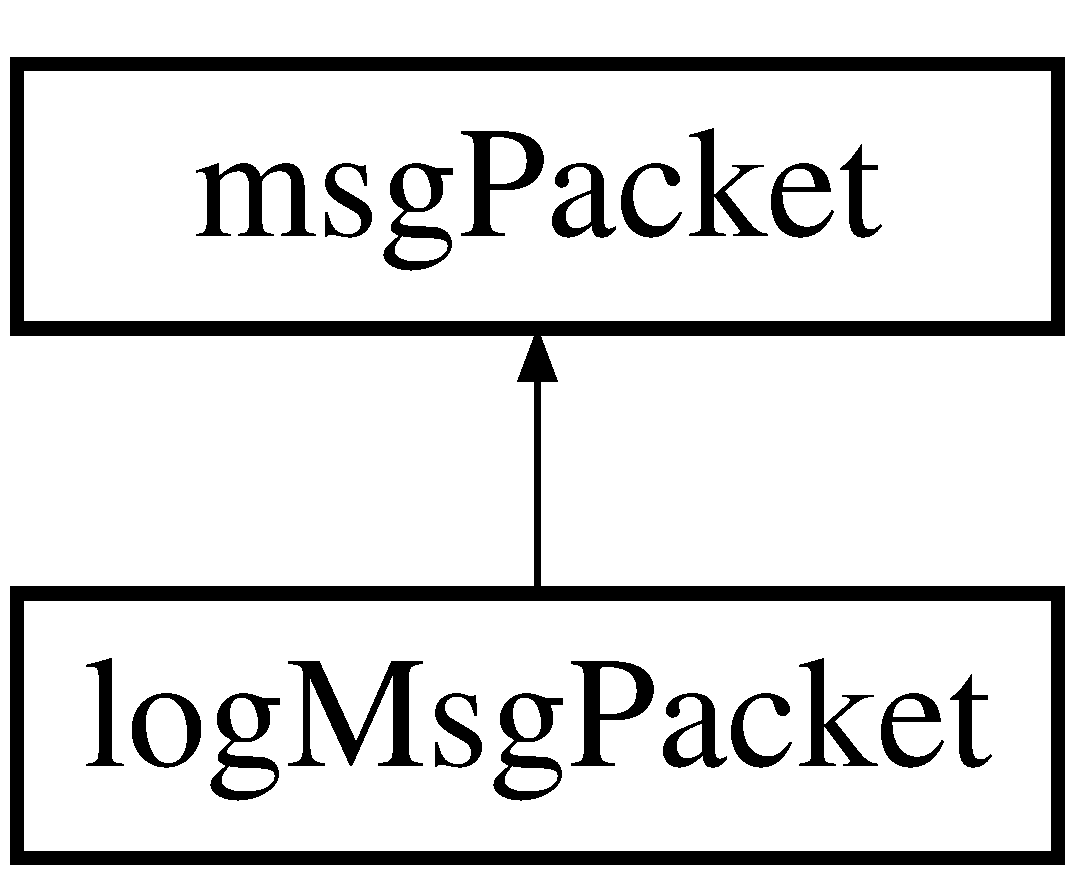
\includegraphics[height=2.000000cm]{structlogMsgPacket}
\end{center}
\end{figure}
\subsection*{Public Member Functions}
\begin{DoxyCompactItemize}
\item 
\hypertarget{structlogMsgPacket_ac6231231cfcd4000902c5bdb3165432c}{\hyperlink{structlogMsgPacket_ac6231231cfcd4000902c5bdb3165432c}{log\-Msg\-Packet} ()}\label{structlogMsgPacket_ac6231231cfcd4000902c5bdb3165432c}

\begin{DoxyCompactList}\small\item\em Default constructor for \hyperlink{structlogMsgPacket}{log\-Msg\-Packet}. \end{DoxyCompactList}\item 
\hyperlink{structlogMsgPacket_ab56f75cef643f8d69b59a007b3e61fa4}{log\-Msg\-Packet} (pid\-\_\-t \hyperlink{structmsgPacket_a294c1f456116eb9177b31ab8b5577f86}{sender}, const char \hyperlink{structmsgPacket_a8b49c124b4ca2ed872692333b71d74fd}{cmd}\mbox{[}$\,$\mbox{]}, char \hyperlink{structlogMsgPacket_a3080c749154c1b7e0f885d5a0bc5859b}{log\-Record}\mbox{[}$\,$\mbox{]})
\begin{DoxyCompactList}\small\item\em Constructs a \hyperlink{structintMsgPacket}{int\-Msg\-Packet} given its elements. \end{DoxyCompactList}\end{DoxyCompactItemize}
\subsection*{Public Attributes}
\begin{DoxyCompactItemize}
\item 
char \hyperlink{structlogMsgPacket_a3080c749154c1b7e0f885d5a0bc5859b}{log\-Record} \mbox{[}\hyperlink{msgPackets_8cpp_a66ac50a388642c37f3908540f06ff1bf}{M\-A\-X\-L\-O\-G\-R\-E\-C\-O\-R\-D\-S\-I\-Z\-E}\mbox{]}
\end{DoxyCompactItemize}


\subsection{Detailed Description}
Sub-\/\-Struct T\-C\-P message packet for transmitting log records. 

\subsection{Constructor \& Destructor Documentation}
\hypertarget{structlogMsgPacket_ab56f75cef643f8d69b59a007b3e61fa4}{\index{log\-Msg\-Packet@{log\-Msg\-Packet}!log\-Msg\-Packet@{log\-Msg\-Packet}}
\index{log\-Msg\-Packet@{log\-Msg\-Packet}!logMsgPacket@{log\-Msg\-Packet}}
\subsubsection[{log\-Msg\-Packet}]{\setlength{\rightskip}{0pt plus 5cm}log\-Msg\-Packet\-::log\-Msg\-Packet (
\begin{DoxyParamCaption}
\item[{pid\-\_\-t}]{sender, }
\item[{const char}]{cmd\mbox{[}$\,$\mbox{]}, }
\item[{char}]{log\-Record\mbox{[}$\,$\mbox{]}}
\end{DoxyParamCaption}
)\hspace{0.3cm}{\ttfamily [inline]}}}\label{structlogMsgPacket_ab56f75cef643f8d69b59a007b3e61fa4}


Constructs a \hyperlink{structintMsgPacket}{int\-Msg\-Packet} given its elements. 


\begin{DoxyParams}{Parameters}
{\em sender} & The sender of the message's P\-I\-D. \\
\hline
{\em cmd} & The command for the message. \\
\hline
{\em log\-Record} & The log record to be transmitted. \\
\hline
\end{DoxyParams}


\subsection{Member Data Documentation}
\hypertarget{structlogMsgPacket_a3080c749154c1b7e0f885d5a0bc5859b}{\index{log\-Msg\-Packet@{log\-Msg\-Packet}!log\-Record@{log\-Record}}
\index{log\-Record@{log\-Record}!logMsgPacket@{log\-Msg\-Packet}}
\subsubsection[{log\-Record}]{\setlength{\rightskip}{0pt plus 5cm}log\-Msg\-Packet\-::log\-Record}}\label{structlogMsgPacket_a3080c749154c1b7e0f885d5a0bc5859b}
The container for the log record string 

The documentation for this struct was generated from the following file\-:\begin{DoxyCompactItemize}
\item 
\hyperlink{msgPackets_8cpp}{msg\-Packets.\-cpp}\end{DoxyCompactItemize}

\hypertarget{structmsgPacket}{\section{msg\-Packet Struct Reference}
\label{structmsgPacket}\index{msg\-Packet@{msg\-Packet}}
}


Base Struct T\-C\-P message packet.  


Inheritance diagram for msg\-Packet\-:\begin{figure}[H]
\begin{center}
\leavevmode
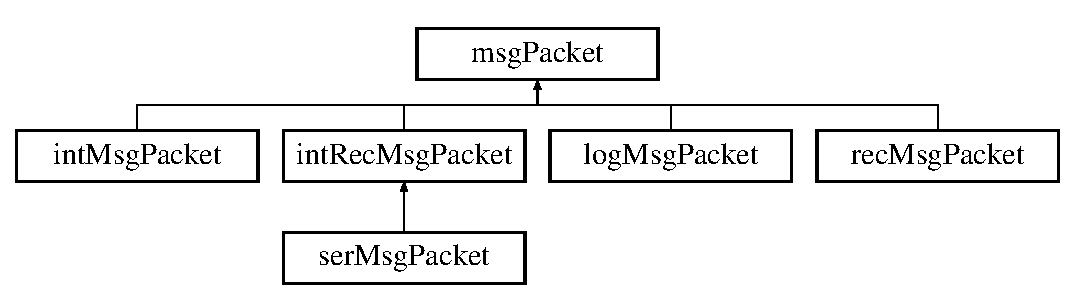
\includegraphics[height=3.000000cm]{structmsgPacket}
\end{center}
\end{figure}
\subsection*{Public Member Functions}
\begin{DoxyCompactItemize}
\item 
\hypertarget{structmsgPacket_aac8ce5e662b88e38544d28343f1bf958}{\hyperlink{structmsgPacket_aac8ce5e662b88e38544d28343f1bf958}{msg\-Packet} ()}\label{structmsgPacket_aac8ce5e662b88e38544d28343f1bf958}

\begin{DoxyCompactList}\small\item\em Default constructor for \hyperlink{structmsgPacket}{msg\-Packet}. \end{DoxyCompactList}\item 
\hyperlink{structmsgPacket_ae7028f6d63c23ee4aca24e863f629ba3}{msg\-Packet} (pid\-\_\-t \hyperlink{structmsgPacket_a294c1f456116eb9177b31ab8b5577f86}{sender}, const char \hyperlink{structmsgPacket_a8b49c124b4ca2ed872692333b71d74fd}{cmd}\mbox{[}$\,$\mbox{]})
\begin{DoxyCompactList}\small\item\em Constructs a \hyperlink{structmsgPacket}{msg\-Packet} given its elements. \end{DoxyCompactList}\end{DoxyCompactItemize}
\subsection*{Public Attributes}
\begin{DoxyCompactItemize}
\item 
pid\-\_\-t \hyperlink{structmsgPacket_a294c1f456116eb9177b31ab8b5577f86}{sender}
\item 
char \hyperlink{structmsgPacket_a8b49c124b4ca2ed872692333b71d74fd}{cmd} \mbox{[}4\mbox{]}
\end{DoxyCompactItemize}


\subsection{Detailed Description}
Base Struct T\-C\-P message packet. 

\subsection{Constructor \& Destructor Documentation}
\hypertarget{structmsgPacket_ae7028f6d63c23ee4aca24e863f629ba3}{\index{msg\-Packet@{msg\-Packet}!msg\-Packet@{msg\-Packet}}
\index{msg\-Packet@{msg\-Packet}!msgPacket@{msg\-Packet}}
\subsubsection[{msg\-Packet}]{\setlength{\rightskip}{0pt plus 5cm}msg\-Packet\-::msg\-Packet (
\begin{DoxyParamCaption}
\item[{pid\-\_\-t}]{sender, }
\item[{const char}]{cmd\mbox{[}$\,$\mbox{]}}
\end{DoxyParamCaption}
)\hspace{0.3cm}{\ttfamily [inline]}}}\label{structmsgPacket_ae7028f6d63c23ee4aca24e863f629ba3}


Constructs a \hyperlink{structmsgPacket}{msg\-Packet} given its elements. 


\begin{DoxyParams}{Parameters}
{\em sender} & The sender of the message's P\-I\-D. \\
\hline
{\em cmd} & The command for the message. \\
\hline
\end{DoxyParams}


\subsection{Member Data Documentation}
\hypertarget{structmsgPacket_a8b49c124b4ca2ed872692333b71d74fd}{\index{msg\-Packet@{msg\-Packet}!cmd@{cmd}}
\index{cmd@{cmd}!msgPacket@{msg\-Packet}}
\subsubsection[{cmd}]{\setlength{\rightskip}{0pt plus 5cm}msg\-Packet\-::cmd}}\label{structmsgPacket_a8b49c124b4ca2ed872692333b71d74fd}
The command for the message \hypertarget{structmsgPacket_a294c1f456116eb9177b31ab8b5577f86}{\index{msg\-Packet@{msg\-Packet}!sender@{sender}}
\index{sender@{sender}!msgPacket@{msg\-Packet}}
\subsubsection[{sender}]{\setlength{\rightskip}{0pt plus 5cm}msg\-Packet\-::sender}}\label{structmsgPacket_a294c1f456116eb9177b31ab8b5577f86}
The pid of the sender of the message 

The documentation for this struct was generated from the following file\-:\begin{DoxyCompactItemize}
\item 
\hyperlink{msgPackets_8cpp}{msg\-Packets.\-cpp}\end{DoxyCompactItemize}

\input{structrecMsgPacket}
\hypertarget{classSemaphoreSet}{\section{Semaphore\-Set Class Reference}
\label{classSemaphoreSet}\index{Semaphore\-Set@{Semaphore\-Set}}
}


Wrapper Class for U\-N\-I\-X System V Semaphores.  


\subsection*{Public Member Functions}
\begin{DoxyCompactItemize}
\item 
\hypertarget{classSemaphoreSet_a91bfe49df662dc06f43dfe9149470fae}{\hyperlink{classSemaphoreSet_a91bfe49df662dc06f43dfe9149470fae}{Semaphore\-Set} ()}\label{classSemaphoreSet_a91bfe49df662dc06f43dfe9149470fae}

\begin{DoxyCompactList}\small\item\em Default constructor for the semaphore set. \end{DoxyCompactList}\item 
\hyperlink{classSemaphoreSet_a11f8c507a74d0d4295f2f9a83943f07a}{Semaphore\-Set} (int key, int num\-Sems, int perm\-Flags)
\begin{DoxyCompactList}\small\item\em Constructs a semaphore set. \end{DoxyCompactList}\item 
\hypertarget{classSemaphoreSet_a8746a1881e8b356db387325e12716116}{void \hyperlink{classSemaphoreSet_a8746a1881e8b356db387325e12716116}{close} ()}\label{classSemaphoreSet_a8746a1881e8b356db387325e12716116}

\begin{DoxyCompactList}\small\item\em Destroys the semaphore set. \end{DoxyCompactList}\item 
int \hyperlink{classSemaphoreSet_a6b1eca22231adc51209113a7e0e1d1e7}{add\-Semaphore} ()
\begin{DoxyCompactList}\small\item\em Adds a semaphore to the semaphore set. \end{DoxyCompactList}\item 
int \hyperlink{classSemaphoreSet_a3d6ae6868cfe3c052dfbd13f2913b036}{remove\-Semaphore} ()
\begin{DoxyCompactList}\small\item\em Removes a semaphore to the semaphore set. \end{DoxyCompactList}\item 
int \hyperlink{classSemaphoreSet_a835d01b6d87fddf4fcb452f2467153e5}{wait} (unsigned short sem\-Num)
\begin{DoxyCompactList}\small\item\em Issues a wait operation on the semaphore. \end{DoxyCompactList}\item 
int \hyperlink{classSemaphoreSet_a81f3eaf327c4ed2547a0962c9be52374}{signal} (unsigned short sem\-Num)
\begin{DoxyCompactList}\small\item\em Signals a semaphore to wakeup a process. \end{DoxyCompactList}\item 
unsigned short $\ast$ \hyperlink{classSemaphoreSet_a80a6f8e9c61a85c366ec61d290928d06}{get\-All} ()
\begin{DoxyCompactList}\small\item\em Retrives the value of all semaphores in the set. \end{DoxyCompactList}\item 
int \hyperlink{classSemaphoreSet_a80e1e53c0eb29c548c1d24556b0f8f9a}{set\-All} (int val)
\begin{DoxyCompactList}\small\item\em Sets the value of all semaphores in the set to the specified value. \end{DoxyCompactList}\item 
unsigned short \hyperlink{classSemaphoreSet_afe106fd82de68de0ba255c351c474580}{get} (unsigned short sem\-Num)
\begin{DoxyCompactList}\small\item\em Gets the value of a single semaphore in the set. \end{DoxyCompactList}\item 
int \hyperlink{classSemaphoreSet_a2cc2c35fa5bb513bc31a565d5a719111}{set} (unsigned short sem\-Num, int val)
\begin{DoxyCompactList}\small\item\em Sets the value of a single semaphore in the set. \end{DoxyCompactList}\item 
int \hyperlink{classSemaphoreSet_ad57c754f58ff0f870c2fe773768f7b18}{get\-Wait\-Count} (unsigned short sem\-Num)
\begin{DoxyCompactList}\small\item\em Returns the number of processes waiting for the semaphore to increase its value. \end{DoxyCompactList}\item 
int \hyperlink{classSemaphoreSet_a01eff4e0d666877dfce9892e0f53de36}{get\-Num\-Sems} ()
\begin{DoxyCompactList}\small\item\em Gets the number of semaphores in the set. \end{DoxyCompactList}\item 
void \hyperlink{classSemaphoreSet_af02b517be7efef6c5baebcf75391d757}{print} ()
\begin{DoxyCompactList}\small\item\em Prints the values of the semaphore set. \end{DoxyCompactList}\end{DoxyCompactItemize}


\subsection{Detailed Description}
Wrapper Class for U\-N\-I\-X System V Semaphores. 

\subsection{Constructor \& Destructor Documentation}
\hypertarget{classSemaphoreSet_a11f8c507a74d0d4295f2f9a83943f07a}{\index{Semaphore\-Set@{Semaphore\-Set}!Semaphore\-Set@{Semaphore\-Set}}
\index{Semaphore\-Set@{Semaphore\-Set}!SemaphoreSet@{Semaphore\-Set}}
\subsubsection[{Semaphore\-Set}]{\setlength{\rightskip}{0pt plus 5cm}Semaphore\-Set\-::\-Semaphore\-Set (
\begin{DoxyParamCaption}
\item[{int}]{key, }
\item[{int}]{num\-Sems, }
\item[{int}]{perm\-Flags}
\end{DoxyParamCaption}
)\hspace{0.3cm}{\ttfamily [inline]}}}\label{classSemaphoreSet_a11f8c507a74d0d4295f2f9a83943f07a}


Constructs a semaphore set. 


\begin{DoxyParams}{Parameters}
{\em key} & The key for the semaphore set. \\
\hline
{\em num\-Sems} & The number of semaphore to create. \\
\hline
{\em perm\-Flags} & The permissions flags for the semaphore set. \\
\hline
\end{DoxyParams}
\begin{DoxyReturn}{Returns}
The semaphore set identifier (0 indicates semaphore set already created, negative value means semaphore set does not exist). 
\end{DoxyReturn}


\subsection{Member Function Documentation}
\hypertarget{classSemaphoreSet_a6b1eca22231adc51209113a7e0e1d1e7}{\index{Semaphore\-Set@{Semaphore\-Set}!add\-Semaphore@{add\-Semaphore}}
\index{add\-Semaphore@{add\-Semaphore}!SemaphoreSet@{Semaphore\-Set}}
\subsubsection[{add\-Semaphore}]{\setlength{\rightskip}{0pt plus 5cm}int Semaphore\-Set\-::add\-Semaphore (
\begin{DoxyParamCaption}
{}
\end{DoxyParamCaption}
)\hspace{0.3cm}{\ttfamily [inline]}}}\label{classSemaphoreSet_a6b1eca22231adc51209113a7e0e1d1e7}


Adds a semaphore to the semaphore set. 

\begin{DoxyReturn}{Returns}
The new semaphore set identifier. 
\end{DoxyReturn}
\hypertarget{classSemaphoreSet_afe106fd82de68de0ba255c351c474580}{\index{Semaphore\-Set@{Semaphore\-Set}!get@{get}}
\index{get@{get}!SemaphoreSet@{Semaphore\-Set}}
\subsubsection[{get}]{\setlength{\rightskip}{0pt plus 5cm}unsigned short Semaphore\-Set\-::get (
\begin{DoxyParamCaption}
\item[{unsigned short}]{sem\-Num}
\end{DoxyParamCaption}
)\hspace{0.3cm}{\ttfamily [inline]}}}\label{classSemaphoreSet_afe106fd82de68de0ba255c351c474580}


Gets the value of a single semaphore in the set. 


\begin{DoxyParams}{Parameters}
{\em sem\-Num} & The number of the semaphore for which to retrieve its value. \\
\hline
\end{DoxyParams}
\begin{DoxyReturn}{Returns}
The value of the specified semaphore. 
\end{DoxyReturn}
\hypertarget{classSemaphoreSet_a80a6f8e9c61a85c366ec61d290928d06}{\index{Semaphore\-Set@{Semaphore\-Set}!get\-All@{get\-All}}
\index{get\-All@{get\-All}!SemaphoreSet@{Semaphore\-Set}}
\subsubsection[{get\-All}]{\setlength{\rightskip}{0pt plus 5cm}unsigned short$\ast$ Semaphore\-Set\-::get\-All (
\begin{DoxyParamCaption}
{}
\end{DoxyParamCaption}
)\hspace{0.3cm}{\ttfamily [inline]}}}\label{classSemaphoreSet_a80a6f8e9c61a85c366ec61d290928d06}


Retrives the value of all semaphores in the set. 

\begin{DoxyReturn}{Returns}
The array of semaphore values on success, N\-U\-L\-L on failure. 
\end{DoxyReturn}
\hypertarget{classSemaphoreSet_a01eff4e0d666877dfce9892e0f53de36}{\index{Semaphore\-Set@{Semaphore\-Set}!get\-Num\-Sems@{get\-Num\-Sems}}
\index{get\-Num\-Sems@{get\-Num\-Sems}!SemaphoreSet@{Semaphore\-Set}}
\subsubsection[{get\-Num\-Sems}]{\setlength{\rightskip}{0pt plus 5cm}int Semaphore\-Set\-::get\-Num\-Sems (
\begin{DoxyParamCaption}
{}
\end{DoxyParamCaption}
)\hspace{0.3cm}{\ttfamily [inline]}}}\label{classSemaphoreSet_a01eff4e0d666877dfce9892e0f53de36}


Gets the number of semaphores in the set. 

\begin{DoxyReturn}{Returns}
The number of semaphores in the set. 
\end{DoxyReturn}
\hypertarget{classSemaphoreSet_ad57c754f58ff0f870c2fe773768f7b18}{\index{Semaphore\-Set@{Semaphore\-Set}!get\-Wait\-Count@{get\-Wait\-Count}}
\index{get\-Wait\-Count@{get\-Wait\-Count}!SemaphoreSet@{Semaphore\-Set}}
\subsubsection[{get\-Wait\-Count}]{\setlength{\rightskip}{0pt plus 5cm}int Semaphore\-Set\-::get\-Wait\-Count (
\begin{DoxyParamCaption}
\item[{unsigned short}]{sem\-Num}
\end{DoxyParamCaption}
)\hspace{0.3cm}{\ttfamily [inline]}}}\label{classSemaphoreSet_ad57c754f58ff0f870c2fe773768f7b18}


Returns the number of processes waiting for the semaphore to increase its value. 


\begin{DoxyParams}{Parameters}
{\em sem\-Num} & The semaphore for which to retrieve the number of waiting processes. \\
\hline
\end{DoxyParams}
\begin{DoxyReturn}{Returns}
The number of processes waiting for the semaphore to increase its value. 
\end{DoxyReturn}
\hypertarget{classSemaphoreSet_af02b517be7efef6c5baebcf75391d757}{\index{Semaphore\-Set@{Semaphore\-Set}!print@{print}}
\index{print@{print}!SemaphoreSet@{Semaphore\-Set}}
\subsubsection[{print}]{\setlength{\rightskip}{0pt plus 5cm}void Semaphore\-Set\-::print (
\begin{DoxyParamCaption}
{}
\end{DoxyParamCaption}
)\hspace{0.3cm}{\ttfamily [inline]}}}\label{classSemaphoreSet_af02b517be7efef6c5baebcf75391d757}


Prints the values of the semaphore set. 

\begin{DoxyAuthor}{Author}
Dr. Daniel Spiegel (source\-: shmdemo.\-cpp) Modified by\-: Griffin Nye 
\end{DoxyAuthor}
\hypertarget{classSemaphoreSet_a3d6ae6868cfe3c052dfbd13f2913b036}{\index{Semaphore\-Set@{Semaphore\-Set}!remove\-Semaphore@{remove\-Semaphore}}
\index{remove\-Semaphore@{remove\-Semaphore}!SemaphoreSet@{Semaphore\-Set}}
\subsubsection[{remove\-Semaphore}]{\setlength{\rightskip}{0pt plus 5cm}int Semaphore\-Set\-::remove\-Semaphore (
\begin{DoxyParamCaption}
{}
\end{DoxyParamCaption}
)\hspace{0.3cm}{\ttfamily [inline]}}}\label{classSemaphoreSet_a3d6ae6868cfe3c052dfbd13f2913b036}


Removes a semaphore to the semaphore set. 

\begin{DoxyReturn}{Returns}
The new semaphore set identifier. 
\end{DoxyReturn}
\hypertarget{classSemaphoreSet_a2cc2c35fa5bb513bc31a565d5a719111}{\index{Semaphore\-Set@{Semaphore\-Set}!set@{set}}
\index{set@{set}!SemaphoreSet@{Semaphore\-Set}}
\subsubsection[{set}]{\setlength{\rightskip}{0pt plus 5cm}int Semaphore\-Set\-::set (
\begin{DoxyParamCaption}
\item[{unsigned short}]{sem\-Num, }
\item[{int}]{val}
\end{DoxyParamCaption}
)\hspace{0.3cm}{\ttfamily [inline]}}}\label{classSemaphoreSet_a2cc2c35fa5bb513bc31a565d5a719111}


Sets the value of a single semaphore in the set. 


\begin{DoxyParams}{Parameters}
{\em sem\-Num} & The number of the semaphore for which to set its value. \\
\hline
{\em val} & The value to set the semaphore to. \\
\hline
\end{DoxyParams}
\begin{DoxyReturn}{Returns}
0 on success, -\/1 on failure. 
\end{DoxyReturn}
\hypertarget{classSemaphoreSet_a80e1e53c0eb29c548c1d24556b0f8f9a}{\index{Semaphore\-Set@{Semaphore\-Set}!set\-All@{set\-All}}
\index{set\-All@{set\-All}!SemaphoreSet@{Semaphore\-Set}}
\subsubsection[{set\-All}]{\setlength{\rightskip}{0pt plus 5cm}int Semaphore\-Set\-::set\-All (
\begin{DoxyParamCaption}
\item[{int}]{val}
\end{DoxyParamCaption}
)\hspace{0.3cm}{\ttfamily [inline]}}}\label{classSemaphoreSet_a80e1e53c0eb29c548c1d24556b0f8f9a}


Sets the value of all semaphores in the set to the specified value. 


\begin{DoxyParams}{Parameters}
{\em val} & The value to set all semaphores in the set to. \\
\hline
\end{DoxyParams}
\begin{DoxyReturn}{Returns}
0 on success, -\/1 on failure. 
\end{DoxyReturn}
\hypertarget{classSemaphoreSet_a81f3eaf327c4ed2547a0962c9be52374}{\index{Semaphore\-Set@{Semaphore\-Set}!signal@{signal}}
\index{signal@{signal}!SemaphoreSet@{Semaphore\-Set}}
\subsubsection[{signal}]{\setlength{\rightskip}{0pt plus 5cm}int Semaphore\-Set\-::signal (
\begin{DoxyParamCaption}
\item[{unsigned short}]{sem\-Num}
\end{DoxyParamCaption}
)\hspace{0.3cm}{\ttfamily [inline]}}}\label{classSemaphoreSet_a81f3eaf327c4ed2547a0962c9be52374}


Signals a semaphore to wakeup a process. 


\begin{DoxyParams}{Parameters}
{\em sem\-Num} & The semaphore to issue the signal to. \\
\hline
\end{DoxyParams}
\begin{DoxyReturn}{Returns}
0 on success, -\/1 on failure. 
\end{DoxyReturn}
\hypertarget{classSemaphoreSet_a835d01b6d87fddf4fcb452f2467153e5}{\index{Semaphore\-Set@{Semaphore\-Set}!wait@{wait}}
\index{wait@{wait}!SemaphoreSet@{Semaphore\-Set}}
\subsubsection[{wait}]{\setlength{\rightskip}{0pt plus 5cm}int Semaphore\-Set\-::wait (
\begin{DoxyParamCaption}
\item[{unsigned short}]{sem\-Num}
\end{DoxyParamCaption}
)\hspace{0.3cm}{\ttfamily [inline]}}}\label{classSemaphoreSet_a835d01b6d87fddf4fcb452f2467153e5}


Issues a wait operation on the semaphore. 


\begin{DoxyParams}{Parameters}
{\em sem\-Num} & The semaphore to issue the wait operation to. \\
\hline
\end{DoxyParams}
\begin{DoxyReturn}{Returns}
0 on success, -\/1 on failure. 
\end{DoxyReturn}


The documentation for this class was generated from the following file\-:\begin{DoxyCompactItemize}
\item 
\hyperlink{SemaphoreSet_8cpp}{Semaphore\-Set.\-cpp}\end{DoxyCompactItemize}

\hypertarget{structserMsgPacket}{\section{ser\-Msg\-Packet Struct Reference}
\label{structserMsgPacket}\index{ser\-Msg\-Packet@{ser\-Msg\-Packet}}
}


Union Struct T\-C\-P message packet for receiving messages on server side.  


Inheritance diagram for ser\-Msg\-Packet\-:\begin{figure}[H]
\begin{center}
\leavevmode
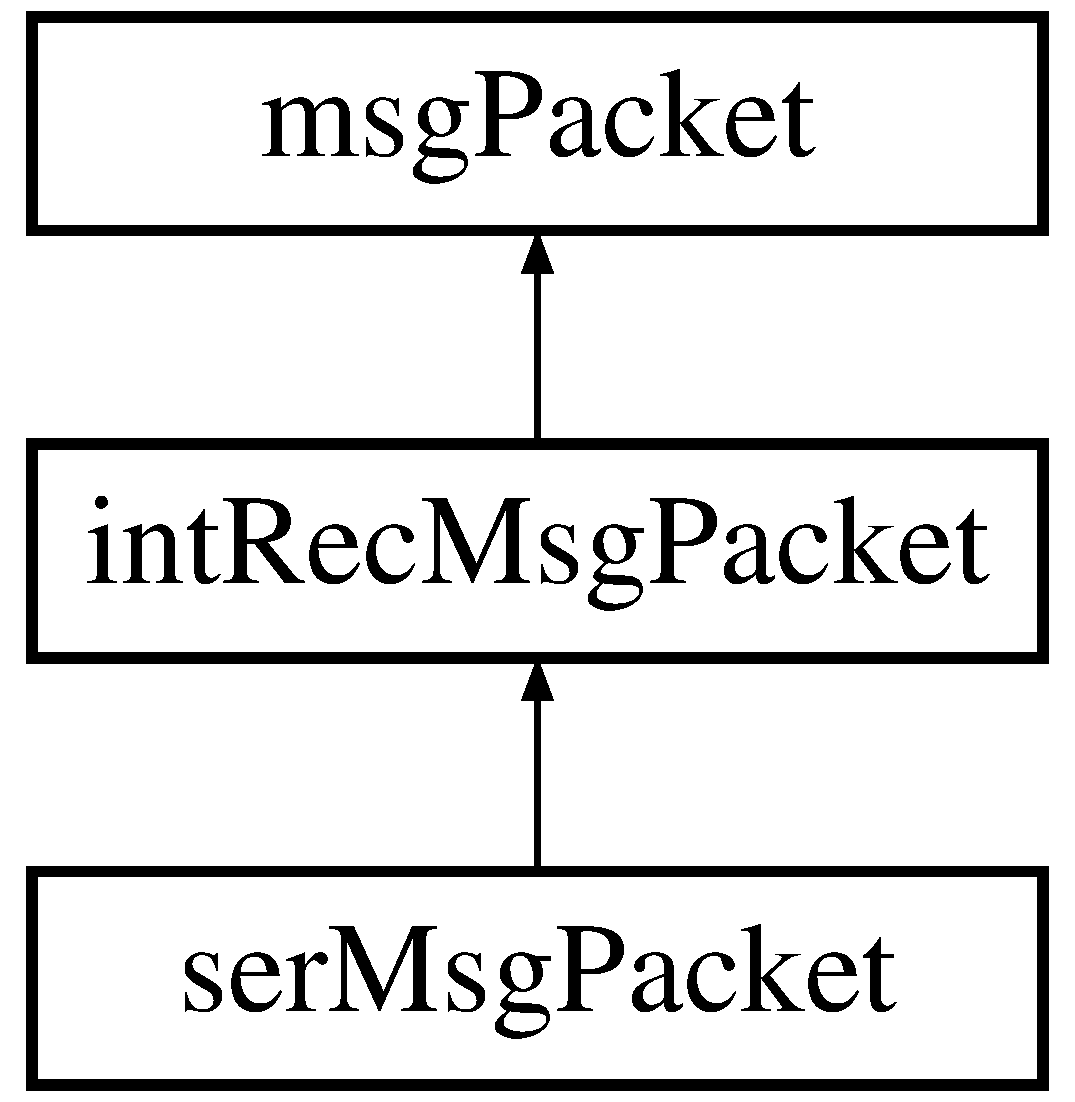
\includegraphics[height=3.000000cm]{structserMsgPacket}
\end{center}
\end{figure}
\subsection*{Public Member Functions}
\begin{DoxyCompactItemize}
\item 
\hypertarget{structserMsgPacket_a5b29522ee436c31160f86b4d73504069}{\hyperlink{structserMsgPacket_a5b29522ee436c31160f86b4d73504069}{ser\-Msg\-Packet} ()}\label{structserMsgPacket_a5b29522ee436c31160f86b4d73504069}

\begin{DoxyCompactList}\small\item\em Default constructor for \hyperlink{structserMsgPacket}{ser\-Msg\-Packet}. \end{DoxyCompactList}\item 
\hyperlink{structserMsgPacket_a19c1ff1a31f9adca56023d59fde6c428}{ser\-Msg\-Packet} (pid\-\_\-t \hyperlink{structmsgPacket_a294c1f456116eb9177b31ab8b5577f86}{sender}, const char \hyperlink{structmsgPacket_a8b49c124b4ca2ed872692333b71d74fd}{cmd}\mbox{[}$\,$\mbox{]}, int \hyperlink{structintRecMsgPacket_a09009e50e4f452b7fea038fcb5f8e382}{val}, char \hyperlink{structintRecMsgPacket_a4edab3e169d3d5d2ceced40d663e8055}{record}\mbox{[}$\,$\mbox{]})
\begin{DoxyCompactList}\small\item\em Constructs a \hyperlink{structserMsgPacket}{ser\-Msg\-Packet} given its elements. \end{DoxyCompactList}\end{DoxyCompactItemize}
\subsection*{Additional Inherited Members}


\subsection{Detailed Description}
Union Struct T\-C\-P message packet for receiving messages on server side. 

\subsection{Constructor \& Destructor Documentation}
\hypertarget{structserMsgPacket_a19c1ff1a31f9adca56023d59fde6c428}{\index{ser\-Msg\-Packet@{ser\-Msg\-Packet}!ser\-Msg\-Packet@{ser\-Msg\-Packet}}
\index{ser\-Msg\-Packet@{ser\-Msg\-Packet}!serMsgPacket@{ser\-Msg\-Packet}}
\subsubsection[{ser\-Msg\-Packet}]{\setlength{\rightskip}{0pt plus 5cm}ser\-Msg\-Packet\-::ser\-Msg\-Packet (
\begin{DoxyParamCaption}
\item[{pid\-\_\-t}]{sender, }
\item[{const char}]{cmd\mbox{[}$\,$\mbox{]}, }
\item[{int}]{val, }
\item[{char}]{record\mbox{[}$\,$\mbox{]}}
\end{DoxyParamCaption}
)\hspace{0.3cm}{\ttfamily [inline]}}}\label{structserMsgPacket_a19c1ff1a31f9adca56023d59fde6c428}


Constructs a \hyperlink{structserMsgPacket}{ser\-Msg\-Packet} given its elements. 


\begin{DoxyParams}{Parameters}
{\em sender} & The sender of the message's P\-I\-D. \\
\hline
{\em cmd} & The command for the message. \\
\hline
{\em val} & The record count or record index to be transmitted in the message. \\
\hline
{\em record} & The record to be transmitted in the message. \\
\hline
\end{DoxyParams}


The documentation for this struct was generated from the following file\-:\begin{DoxyCompactItemize}
\item 
\hyperlink{msgPackets_8cpp}{msg\-Packets.\-cpp}\end{DoxyCompactItemize}

\hypertarget{structSharedMemoryManager_1_1sharedMemBlock}{\section{Shared\-Memory\-Manager\-:\-:shared\-Mem\-Block Struct Reference}
\label{structSharedMemoryManager_1_1sharedMemBlock}\index{Shared\-Memory\-Manager\-::shared\-Mem\-Block@{Shared\-Memory\-Manager\-::shared\-Mem\-Block}}
}


Container struct of all fields in a client process' shared memory block.  


\subsection*{Public Attributes}
\begin{DoxyCompactItemize}
\item 
pid\-\_\-t \hyperlink{structSharedMemoryManager_1_1sharedMemBlock_af10ab35d9c14b164824710adeb4bb2ef}{pid}
\item 
system\-\_\-clock\-::time\-\_\-point \hyperlink{structSharedMemoryManager_1_1sharedMemBlock_a91e99382dfd3baa0a9e9864f0c9964e1}{start\-Time}
\item 
int \hyperlink{structSharedMemoryManager_1_1sharedMemBlock_aa3562377afe5f7cb1294887bd328437f}{num\-Commands}
\item 
system\-\_\-clock\-::time\-\_\-point \hyperlink{structSharedMemoryManager_1_1sharedMemBlock_a83d99997177411ee92117b99b1924ddf}{last\-Msg\-Time}
\end{DoxyCompactItemize}


\subsection{Detailed Description}
Container struct of all fields in a client process' shared memory block. 

\subsection{Member Data Documentation}
\hypertarget{structSharedMemoryManager_1_1sharedMemBlock_a83d99997177411ee92117b99b1924ddf}{\index{Shared\-Memory\-Manager\-::shared\-Mem\-Block@{Shared\-Memory\-Manager\-::shared\-Mem\-Block}!last\-Msg\-Time@{last\-Msg\-Time}}
\index{last\-Msg\-Time@{last\-Msg\-Time}!SharedMemoryManager::sharedMemBlock@{Shared\-Memory\-Manager\-::shared\-Mem\-Block}}
\subsubsection[{last\-Msg\-Time}]{\setlength{\rightskip}{0pt plus 5cm}Shared\-Memory\-Manager\-::shared\-Mem\-Block\-::last\-Msg\-Time}}\label{structSharedMemoryManager_1_1sharedMemBlock_a83d99997177411ee92117b99b1924ddf}
The current system time when the client process last issued a command. \hypertarget{structSharedMemoryManager_1_1sharedMemBlock_aa3562377afe5f7cb1294887bd328437f}{\index{Shared\-Memory\-Manager\-::shared\-Mem\-Block@{Shared\-Memory\-Manager\-::shared\-Mem\-Block}!num\-Commands@{num\-Commands}}
\index{num\-Commands@{num\-Commands}!SharedMemoryManager::sharedMemBlock@{Shared\-Memory\-Manager\-::shared\-Mem\-Block}}
\subsubsection[{num\-Commands}]{\setlength{\rightskip}{0pt plus 5cm}Shared\-Memory\-Manager\-::shared\-Mem\-Block\-::num\-Commands}}\label{structSharedMemoryManager_1_1sharedMemBlock_aa3562377afe5f7cb1294887bd328437f}
The number of commands this client process has issued to the server. \hypertarget{structSharedMemoryManager_1_1sharedMemBlock_af10ab35d9c14b164824710adeb4bb2ef}{\index{Shared\-Memory\-Manager\-::shared\-Mem\-Block@{Shared\-Memory\-Manager\-::shared\-Mem\-Block}!pid@{pid}}
\index{pid@{pid}!SharedMemoryManager::sharedMemBlock@{Shared\-Memory\-Manager\-::shared\-Mem\-Block}}
\subsubsection[{pid}]{\setlength{\rightskip}{0pt plus 5cm}Shared\-Memory\-Manager\-::shared\-Mem\-Block\-::pid}}\label{structSharedMemoryManager_1_1sharedMemBlock_af10ab35d9c14b164824710adeb4bb2ef}
The pid of the client process using this block of shared memory. \hypertarget{structSharedMemoryManager_1_1sharedMemBlock_a91e99382dfd3baa0a9e9864f0c9964e1}{\index{Shared\-Memory\-Manager\-::shared\-Mem\-Block@{Shared\-Memory\-Manager\-::shared\-Mem\-Block}!start\-Time@{start\-Time}}
\index{start\-Time@{start\-Time}!SharedMemoryManager::sharedMemBlock@{Shared\-Memory\-Manager\-::shared\-Mem\-Block}}
\subsubsection[{start\-Time}]{\setlength{\rightskip}{0pt plus 5cm}Shared\-Memory\-Manager\-::shared\-Mem\-Block\-::start\-Time}}\label{structSharedMemoryManager_1_1sharedMemBlock_a91e99382dfd3baa0a9e9864f0c9964e1}
The current system time at the time of the client process' execution. 

The documentation for this struct was generated from the following file\-:\begin{DoxyCompactItemize}
\item 
\hyperlink{SharedMemoryManager_8cpp}{Shared\-Memory\-Manager.\-cpp}\end{DoxyCompactItemize}

\hypertarget{classSharedMemoryManager}{\section{Shared\-Memory\-Manager Class Reference}
\label{classSharedMemoryManager}\index{Shared\-Memory\-Manager@{Shared\-Memory\-Manager}}
}


Wrapper\-Class Implementation of U\-N\-I\-X Shared Memory for easier creation, storage, and retrieval.  


\subsection*{Classes}
\begin{DoxyCompactItemize}
\item 
struct \hyperlink{structSharedMemoryManager_1_1sharedMemBlock}{shared\-Mem\-Block}
\begin{DoxyCompactList}\small\item\em Container struct of all fields in a client process' shared memory block. \end{DoxyCompactList}\end{DoxyCompactItemize}
\subsection*{Public Member Functions}
\begin{DoxyCompactItemize}
\item 
struct \\*
\hyperlink{structSharedMemoryManager_1_1sharedMemBlock}{Shared\-Memory\-Manager\-::shared\-Mem\-Block} \hyperlink{classSharedMemoryManager_a30d8438be6747a19fc23450514445cab}{Shared\-Memory\-Manager} (int key, int perms)
\begin{DoxyCompactList}\small\item\em Allocates the shared memory space and constructs the Shared\-Memory object. \end{DoxyCompactList}\item 
void $\ast$ \hyperlink{classSharedMemoryManager_a4118ad7e39bcb21bc858cd4b307a830e}{attach} ()
\begin{DoxyCompactList}\small\item\em Attaches the first open shared memory address to the calling process. \end{DoxyCompactList}\item 
bool \hyperlink{classSharedMemoryManager_a5c8eb92892c13e1e3007d236d538c8e7}{detach} ()
\begin{DoxyCompactList}\small\item\em Detaches the shared memory space from the calling process. \end{DoxyCompactList}\item 
bool \hyperlink{classSharedMemoryManager_a95d1f28eb377b4988dcf1724dcffe946}{destroy} ()
\begin{DoxyCompactList}\small\item\em Destroys the shared memory space. (N\-O\-T\-E\-: This is N\-O\-T a destructor for the Shared\-Memory object, however, calling this will render the object useless.) \end{DoxyCompactList}\item 
\hypertarget{classSharedMemoryManager_aed3b566162518064ccca17fa071e64b9}{void \hyperlink{classSharedMemoryManager_aed3b566162518064ccca17fa071e64b9}{increment\-Num\-Clients} ()}\label{classSharedMemoryManager_aed3b566162518064ccca17fa071e64b9}

\begin{DoxyCompactList}\small\item\em Increments the number of clients field in the shared memory space. \end{DoxyCompactList}\item 
\hypertarget{classSharedMemoryManager_a106346050cf61a7f270f078632d510f4}{void \hyperlink{classSharedMemoryManager_a106346050cf61a7f270f078632d510f4}{decrement\-Num\-Clients} ()}\label{classSharedMemoryManager_a106346050cf61a7f270f078632d510f4}

\begin{DoxyCompactList}\small\item\em Decrements the number of clients field in the shared memory space. \end{DoxyCompactList}\item 
void \hyperlink{classSharedMemoryManager_ad598919ed2f1ca742b7f004587403ab8}{init\-Block} (pid\-\_\-t cli\-P\-I\-D)
\begin{DoxyCompactList}\small\item\em Initializes the P\-I\-D and start\-Time fields of the shared memory block and stores the pointer to this block. \end{DoxyCompactList}\item 
\hypertarget{classSharedMemoryManager_afc90af415f4d62609a66db29c2c185cd}{void \hyperlink{classSharedMemoryManager_afc90af415f4d62609a66db29c2c185cd}{clear\-Block} ()}\label{classSharedMemoryManager_afc90af415f4d62609a66db29c2c185cd}

\begin{DoxyCompactList}\small\item\em Clears the calling process' shared memory block. \end{DoxyCompactList}\item 
\hypertarget{classSharedMemoryManager_a7937104b69646b8c1216504d920cc417}{void \hyperlink{classSharedMemoryManager_a7937104b69646b8c1216504d920cc417}{increment\-Command} ()}\label{classSharedMemoryManager_a7937104b69646b8c1216504d920cc417}

\begin{DoxyCompactList}\small\item\em Increments/\-Updates the num\-Command and last\-Msg\-Time fields of the shared memory block. \end{DoxyCompactList}\item 
struct \hyperlink{structSharedMemoryManager_1_1sharedMemBlock}{shared\-Mem\-Block} $\ast$ \hyperlink{classSharedMemoryManager_a3ec080502acf8c32b97024ad65e83724}{find\-Avail\-Block} ()
\begin{DoxyCompactList}\small\item\em Finds the first available shared memory block in the shared memory space. \end{DoxyCompactList}\end{DoxyCompactItemize}


\subsection{Detailed Description}
Wrapper\-Class Implementation of U\-N\-I\-X Shared Memory for easier creation, storage, and retrieval. 

\subsection{Constructor \& Destructor Documentation}
\hypertarget{classSharedMemoryManager_a30d8438be6747a19fc23450514445cab}{\index{Shared\-Memory\-Manager@{Shared\-Memory\-Manager}!Shared\-Memory\-Manager@{Shared\-Memory\-Manager}}
\index{Shared\-Memory\-Manager@{Shared\-Memory\-Manager}!SharedMemoryManager@{Shared\-Memory\-Manager}}
\subsubsection[{Shared\-Memory\-Manager}]{\setlength{\rightskip}{0pt plus 5cm}struct {\bf Shared\-Memory\-Manager\-::shared\-Mem\-Block} Shared\-Memory\-Manager\-::\-Shared\-Memory\-Manager (
\begin{DoxyParamCaption}
\item[{int}]{key, }
\item[{int}]{perms}
\end{DoxyParamCaption}
)\hspace{0.3cm}{\ttfamily [inline]}}}\label{classSharedMemoryManager_a30d8438be6747a19fc23450514445cab}


Allocates the shared memory space and constructs the Shared\-Memory object. 


\begin{DoxyParams}{Parameters}
{\em key} & The key for the shared memory space. \\
\hline
{\em perms} & The permission flags for the shared memory space. \\
\hline
\end{DoxyParams}


\subsection{Member Function Documentation}
\hypertarget{classSharedMemoryManager_a4118ad7e39bcb21bc858cd4b307a830e}{\index{Shared\-Memory\-Manager@{Shared\-Memory\-Manager}!attach@{attach}}
\index{attach@{attach}!SharedMemoryManager@{Shared\-Memory\-Manager}}
\subsubsection[{attach}]{\setlength{\rightskip}{0pt plus 5cm}void$\ast$ Shared\-Memory\-Manager\-::attach (
\begin{DoxyParamCaption}
{}
\end{DoxyParamCaption}
)\hspace{0.3cm}{\ttfamily [inline]}}}\label{classSharedMemoryManager_a4118ad7e39bcb21bc858cd4b307a830e}


Attaches the first open shared memory address to the calling process. 

\begin{DoxyReturn}{Returns}
Pointer to the first byte of the shared memory space. N\-U\-L\-L on failure to attach. 
\end{DoxyReturn}
\hypertarget{classSharedMemoryManager_a95d1f28eb377b4988dcf1724dcffe946}{\index{Shared\-Memory\-Manager@{Shared\-Memory\-Manager}!destroy@{destroy}}
\index{destroy@{destroy}!SharedMemoryManager@{Shared\-Memory\-Manager}}
\subsubsection[{destroy}]{\setlength{\rightskip}{0pt plus 5cm}bool Shared\-Memory\-Manager\-::destroy (
\begin{DoxyParamCaption}
{}
\end{DoxyParamCaption}
)\hspace{0.3cm}{\ttfamily [inline]}}}\label{classSharedMemoryManager_a95d1f28eb377b4988dcf1724dcffe946}


Destroys the shared memory space. (N\-O\-T\-E\-: This is N\-O\-T a destructor for the Shared\-Memory object, however, calling this will render the object useless.) 

\begin{DoxyReturn}{Returns}
Success status of the call. 
\end{DoxyReturn}
\hypertarget{classSharedMemoryManager_a5c8eb92892c13e1e3007d236d538c8e7}{\index{Shared\-Memory\-Manager@{Shared\-Memory\-Manager}!detach@{detach}}
\index{detach@{detach}!SharedMemoryManager@{Shared\-Memory\-Manager}}
\subsubsection[{detach}]{\setlength{\rightskip}{0pt plus 5cm}bool Shared\-Memory\-Manager\-::detach (
\begin{DoxyParamCaption}
{}
\end{DoxyParamCaption}
)\hspace{0.3cm}{\ttfamily [inline]}}}\label{classSharedMemoryManager_a5c8eb92892c13e1e3007d236d538c8e7}


Detaches the shared memory space from the calling process. 

\begin{DoxyReturn}{Returns}
Success status of the call. 
\end{DoxyReturn}
\hypertarget{classSharedMemoryManager_a3ec080502acf8c32b97024ad65e83724}{\index{Shared\-Memory\-Manager@{Shared\-Memory\-Manager}!find\-Avail\-Block@{find\-Avail\-Block}}
\index{find\-Avail\-Block@{find\-Avail\-Block}!SharedMemoryManager@{Shared\-Memory\-Manager}}
\subsubsection[{find\-Avail\-Block}]{\setlength{\rightskip}{0pt plus 5cm}struct {\bf shared\-Mem\-Block}$\ast$ Shared\-Memory\-Manager\-::find\-Avail\-Block (
\begin{DoxyParamCaption}
{}
\end{DoxyParamCaption}
)\hspace{0.3cm}{\ttfamily [inline]}}}\label{classSharedMemoryManager_a3ec080502acf8c32b97024ad65e83724}


Finds the first available shared memory block in the shared memory space. 

\begin{DoxyReturn}{Returns}
The \hyperlink{structSharedMemoryManager_1_1sharedMemBlock}{shared\-Mem\-Block} struct pointer to the first available shared memory block. 
\end{DoxyReturn}
\hypertarget{classSharedMemoryManager_ad598919ed2f1ca742b7f004587403ab8}{\index{Shared\-Memory\-Manager@{Shared\-Memory\-Manager}!init\-Block@{init\-Block}}
\index{init\-Block@{init\-Block}!SharedMemoryManager@{Shared\-Memory\-Manager}}
\subsubsection[{init\-Block}]{\setlength{\rightskip}{0pt plus 5cm}void Shared\-Memory\-Manager\-::init\-Block (
\begin{DoxyParamCaption}
\item[{pid\-\_\-t}]{cli\-P\-I\-D}
\end{DoxyParamCaption}
)\hspace{0.3cm}{\ttfamily [inline]}}}\label{classSharedMemoryManager_ad598919ed2f1ca742b7f004587403ab8}


Initializes the P\-I\-D and start\-Time fields of the shared memory block and stores the pointer to this block. 


\begin{DoxyParams}{Parameters}
{\em cli\-P\-I\-D} & The calling process' P\-I\-D. \\
\hline
\end{DoxyParams}


The documentation for this class was generated from the following file\-:\begin{DoxyCompactItemize}
\item 
\hyperlink{SharedMemoryManager_8cpp}{Shared\-Memory\-Manager.\-cpp}\end{DoxyCompactItemize}

\hypertarget{classstringToMonthConverter}{\section{string\-To\-Month\-Converter Class Reference}
\label{classstringToMonthConverter}\index{string\-To\-Month\-Converter@{string\-To\-Month\-Converter}}
}


Used to map enum values to valid input strings for the month field of new records.  


\subsection*{Public Member Functions}
\begin{DoxyCompactItemize}
\item 
\hypertarget{classstringToMonthConverter_ae4da495454c8fe404cf8b2e7846bcc11}{\hyperlink{classstringToMonthConverter_ae4da495454c8fe404cf8b2e7846bcc11}{string\-To\-Month\-Converter} ()}\label{classstringToMonthConverter_ae4da495454c8fe404cf8b2e7846bcc11}

\begin{DoxyCompactList}\small\item\em Constructor for the \hyperlink{classstringToMonthConverter}{string\-To\-Month\-Converter}. Populates the month\-Map. \end{DoxyCompactList}\item 
bool \hyperlink{classstringToMonthConverter_abc4a5665e84e6a6dc27c24b28a21ecb4}{is\-Month} (string month)
\begin{DoxyCompactList}\small\item\em Returns whether the provided string is a valid 3-\/letter month abbreviation. \end{DoxyCompactList}\end{DoxyCompactItemize}


\subsection{Detailed Description}
Used to map enum values to valid input strings for the month field of new records. 

\subsection{Member Function Documentation}
\hypertarget{classstringToMonthConverter_abc4a5665e84e6a6dc27c24b28a21ecb4}{\index{string\-To\-Month\-Converter@{string\-To\-Month\-Converter}!is\-Month@{is\-Month}}
\index{is\-Month@{is\-Month}!stringToMonthConverter@{string\-To\-Month\-Converter}}
\subsubsection[{is\-Month}]{\setlength{\rightskip}{0pt plus 5cm}bool string\-To\-Month\-Converter\-::is\-Month (
\begin{DoxyParamCaption}
\item[{string}]{month}
\end{DoxyParamCaption}
)\hspace{0.3cm}{\ttfamily [inline]}}}\label{classstringToMonthConverter_abc4a5665e84e6a6dc27c24b28a21ecb4}


Returns whether the provided string is a valid 3-\/letter month abbreviation. 


\begin{DoxyParams}{Parameters}
{\em month} & The string to be checked \\
\hline
\end{DoxyParams}
\begin{DoxyReturn}{Returns}
Whether the string is a valid 3-\/letter month abbreviation 
\end{DoxyReturn}


The documentation for this class was generated from the following file\-:\begin{DoxyCompactItemize}
\item 
\hyperlink{msgPackets_8cpp}{msg\-Packets.\-cpp}\end{DoxyCompactItemize}

\chapter{File Documentation}
\hypertarget{client_8cpp}{\section{client.\-cpp File Reference}
\label{client_8cpp}\index{client.\-cpp@{client.\-cpp}}
}


Client side of the T\-C\-P Distributed Information System implementation C\-S\-C552 Dr. Spiegel Spring 2020.  


{\ttfamily \#include $<$iostream$>$}\\*
{\ttfamily \#include $<$netdb.\-h$>$}\\*
{\ttfamily \#include $<$string$>$}\\*
{\ttfamily \#include $<$sys/socket.\-h$>$}\\*
{\ttfamily \#include $<$unistd.\-h$>$}\\*
{\ttfamily \#include \char`\"{}Data\-Record.\-cpp\char`\"{}}\\*
{\ttfamily \#include \char`\"{}msg\-Packets.\-cpp\char`\"{}}\\*
\subsection*{Functions}
\begin{DoxyCompactItemize}
\item 
void \hyperlink{client_8cpp_a72efaf06056cf96435d100c4e0c0b10a}{change\-Record} (int sockfd, pid\-\_\-t my\-P\-I\-D)
\begin{DoxyCompactList}\small\item\em Handles client-\/server and user-\/client interaction for the Change Record menu option. \end{DoxyCompactList}\item 
int \hyperlink{client_8cpp_abd75338c1858a15572c03bf9ec14c926}{connect} (int S\-E\-R\-V\-E\-R\-\_\-\-P\-O\-R\-T, struct in\-\_\-addr $\ast$S\-E\-R\-V\-E\-R\-\_\-\-A\-D\-D\-R\-E\-S\-S)
\begin{DoxyCompactList}\small\item\em Attempts to connect to the server. Returns socket file descriptor on successful connection. \end{DoxyCompactList}\item 
\hypertarget{client_8cpp_acf1494aaf51500b57c44b9e68b652b8a}{void \hyperlink{client_8cpp_acf1494aaf51500b57c44b9e68b652b8a}{display\-Field\-Menu} ()}\label{client_8cpp_acf1494aaf51500b57c44b9e68b652b8a}

\begin{DoxyCompactList}\small\item\em Displays the menu of editable field options to the user. \end{DoxyCompactList}\item 
\hypertarget{client_8cpp_a59c2926dd9b0968badf463aaf4f91422}{void \hyperlink{client_8cpp_a59c2926dd9b0968badf463aaf4f91422}{display\-Menu} ()}\label{client_8cpp_a59c2926dd9b0968badf463aaf4f91422}

\begin{DoxyCompactList}\small\item\em Displays the Main Menu to the user. \end{DoxyCompactList}\item 
\hyperlink{classDataRecord}{Data\-Record} \hyperlink{client_8cpp_aa22e1b410c58a57567eb507a6e74b809}{display\-Record} (int sockfd, pid\-\_\-t my\-P\-I\-D, bool selected\-Menu\-Option)
\begin{DoxyCompactList}\small\item\em Handles client-\/server and user-\/client interaction for the Display Record menu option. \end{DoxyCompactList}\item 
int \hyperlink{client_8cpp_ae0d8ef995548e0f8b1a6ef542c395664}{get\-Count} (int sockfd, pid\-\_\-t my\-P\-I\-D)
\begin{DoxyCompactList}\small\item\em Handles interaction with server for retrieving the record count. \end{DoxyCompactList}\item 
char \hyperlink{client_8cpp_aa46346f48e3b5f40cd4f8be7c653549f}{get\-Menu\-Input} (bool main\-Menu)
\begin{DoxyCompactList}\small\item\em Retrieves the user's menu selection, prompting again for invalid entries. \end{DoxyCompactList}\item 
void \hyperlink{client_8cpp_a250a004e35b04fb1956b9d8cbccf8846}{new\-Record} (int sockfd, pid\-\_\-t my\-P\-I\-D)
\begin{DoxyCompactList}\small\item\em Handles client-\/server and user-\/client interaction for the New Record menu option. \end{DoxyCompactList}\item 
\hypertarget{client_8cpp_a4bfd094c510aa86a46d596db71f9f43d}{void \hyperlink{client_8cpp_a4bfd094c510aa86a46d596db71f9f43d}{print\-Data\-Labels} ()}\label{client_8cpp_a4bfd094c510aa86a46d596db71f9f43d}

\begin{DoxyCompactList}\small\item\em Prints the data labels for output records. \end{DoxyCompactList}\item 
void \hyperlink{client_8cpp_a9adbdb5939cfbdc54e6b37a90203695a}{print\-Log\-Records} (int sockfd, pid\-\_\-t my\-P\-I\-D, int num\-Records)
\begin{DoxyCompactList}\small\item\em Receives and prints all log records sent by the server. \end{DoxyCompactList}\item 
void \hyperlink{client_8cpp_aff14b7970a9fa9f065e2793772f82a93}{print\-Record} (char record\mbox{[}$\,$\mbox{]})
\begin{DoxyCompactList}\small\item\em Prints the provided record. \end{DoxyCompactList}\item 
float \hyperlink{client_8cpp_a66c0b2a52c5e5660374791878ef03967}{prompt\-Float\-Field} (char field)
\begin{DoxyCompactList}\small\item\em Prompts the user for one of the float fields for a new or updated record. \end{DoxyCompactList}\item 
string \hyperlink{client_8cpp_a37056f14cc3fbb1ef8b70896b6443e1d}{prompt\-Month} ()
\begin{DoxyCompactList}\small\item\em Prompts the user for the month for a new record. Validates input through recursive calls until valid input is given. \end{DoxyCompactList}\item 
\hyperlink{classDataRecord}{Data\-Record} \hyperlink{client_8cpp_a6ec627d475672aff6d9dbd3e078ab318}{prompt\-New\-Record} ()
\begin{DoxyCompactList}\small\item\em Prompts the user to create a new record. \end{DoxyCompactList}\item 
int \hyperlink{client_8cpp_a71314c4b236c0c0323851b154996745d}{prompt\-Sel\-Record} (int num\-Records, bool all\-Records)
\begin{DoxyCompactList}\small\item\em Prompts the user for a record index between 1 and the provided max index. Validates input through recursive calls until valid input is given. \end{DoxyCompactList}\item 
string \hyperlink{client_8cpp_aa34b5cce22d58fd391cacd2166f11dfc}{prompt\-Year} ()
\begin{DoxyCompactList}\small\item\em Prompts the user for the year for a new record. Validates input through recursive calls until valid input is given. \end{DoxyCompactList}\item 
{\footnotesize template$<$class Msg\-Packet $>$ }\\void \hyperlink{client_8cpp_af18ad863f3d64cfe8174182f9eda48ae}{receive\-Msg} (int sockfd, Msg\-Packet \&msg)
\begin{DoxyCompactList}\small\item\em Handles the receipt of messages from the server. \end{DoxyCompactList}\item 
{\footnotesize template$<$class Msg\-Packet $>$ }\\void \hyperlink{client_8cpp_adea406d21c20cfc4ae351f7454cc9e46}{send\-Msg} (int sockfd, Msg\-Packet msg)
\begin{DoxyCompactList}\small\item\em Handles the transmission of messages to the server. \end{DoxyCompactList}\item 
void \hyperlink{client_8cpp_a737f1e9c9e5a3b45d788b8361297175f}{show\-Server\-Log} (int sockfd, pid\-\_\-t my\-P\-I\-D)
\begin{DoxyCompactList}\small\item\em Handles client-\/server and user-\/client interaction for the Show Server Log menu option. \end{DoxyCompactList}\item 
int \hyperlink{client_8cpp_a0ddf1224851353fc92bfbff6f499fa97}{main} (int argc, char $\ast$argv\mbox{[}$\,$\mbox{]})
\begin{DoxyCompactList}\small\item\em Calls the appropriate methods to ensure proper functionality of the client. \end{DoxyCompactList}\end{DoxyCompactItemize}


\subsection{Detailed Description}
Client side of the T\-C\-P Distributed Information System implementation C\-S\-C552 Dr. Spiegel Spring 2020. \begin{DoxyAuthor}{Author}
Griffin Nye 
\end{DoxyAuthor}


\subsection{Function Documentation}
\hypertarget{client_8cpp_a72efaf06056cf96435d100c4e0c0b10a}{\index{client.\-cpp@{client.\-cpp}!change\-Record@{change\-Record}}
\index{change\-Record@{change\-Record}!client.cpp@{client.\-cpp}}
\subsubsection[{change\-Record}]{\setlength{\rightskip}{0pt plus 5cm}void change\-Record (
\begin{DoxyParamCaption}
\item[{int}]{sockfd, }
\item[{pid\-\_\-t}]{my\-P\-I\-D}
\end{DoxyParamCaption}
)}}\label{client_8cpp_a72efaf06056cf96435d100c4e0c0b10a}


Handles client-\/server and user-\/client interaction for the Change Record menu option. 


\begin{DoxyParams}{Parameters}
{\em sockfd} & The currently connected sockets file descriptor. \\
\hline
{\em my\-P\-I\-D} & This client's P\-I\-D. \\
\hline
\end{DoxyParams}
\hypertarget{client_8cpp_abd75338c1858a15572c03bf9ec14c926}{\index{client.\-cpp@{client.\-cpp}!connect@{connect}}
\index{connect@{connect}!client.cpp@{client.\-cpp}}
\subsubsection[{connect}]{\setlength{\rightskip}{0pt plus 5cm}int connect (
\begin{DoxyParamCaption}
\item[{int}]{S\-E\-R\-V\-E\-R\-\_\-\-P\-O\-R\-T, }
\item[{struct in\-\_\-addr $\ast$}]{S\-E\-R\-V\-E\-R\-\_\-\-A\-D\-D\-R\-E\-S\-S}
\end{DoxyParamCaption}
)}}\label{client_8cpp_abd75338c1858a15572c03bf9ec14c926}


Attempts to connect to the server. Returns socket file descriptor on successful connection. 


\begin{DoxyParams}{Parameters}
{\em S\-E\-R\-V\-E\-R\-\_\-\-P\-O\-R\-T} & The server's dedicated port number. \\
\hline
{\em S\-E\-R\-V\-E\-R\-\_\-\-A\-D\-D\-R\-E\-S\-S} & The server's address (stored as in\-\_\-addr). \\
\hline
\end{DoxyParams}
\begin{DoxyReturn}{Returns}
Socket file descriptor on successful connection; client exits on failed connection. 
\end{DoxyReturn}
\hypertarget{client_8cpp_aa22e1b410c58a57567eb507a6e74b809}{\index{client.\-cpp@{client.\-cpp}!display\-Record@{display\-Record}}
\index{display\-Record@{display\-Record}!client.cpp@{client.\-cpp}}
\subsubsection[{display\-Record}]{\setlength{\rightskip}{0pt plus 5cm}{\bf Data\-Record} display\-Record (
\begin{DoxyParamCaption}
\item[{int}]{sockfd, }
\item[{pid\-\_\-t}]{my\-P\-I\-D, }
\item[{bool}]{selected\-Menu\-Option}
\end{DoxyParamCaption}
)}}\label{client_8cpp_aa22e1b410c58a57567eb507a6e74b809}


Handles client-\/server and user-\/client interaction for the Display Record menu option. 


\begin{DoxyParams}{Parameters}
{\em sockfd} & The currently connected socket's file descriptor. \\
\hline
{\em my\-P\-I\-D} & This client's P\-I\-D. \\
\hline
{\em selected\-Menu\-Option} & Whether or not Display Record is the currently selected menu option (false removes -\/999 option). \\
\hline
\end{DoxyParams}
\begin{DoxyReturn}{Returns}
The retrieved record as an instance of \hyperlink{classDataRecord}{Data\-Record}. (Last record retrieved for all records option (-\/999), however the return value is not used in this case). 
\end{DoxyReturn}
\hypertarget{client_8cpp_ae0d8ef995548e0f8b1a6ef542c395664}{\index{client.\-cpp@{client.\-cpp}!get\-Count@{get\-Count}}
\index{get\-Count@{get\-Count}!client.cpp@{client.\-cpp}}
\subsubsection[{get\-Count}]{\setlength{\rightskip}{0pt plus 5cm}int get\-Count (
\begin{DoxyParamCaption}
\item[{int}]{sockfd, }
\item[{pid\-\_\-t}]{my\-P\-I\-D}
\end{DoxyParamCaption}
)}}\label{client_8cpp_ae0d8ef995548e0f8b1a6ef542c395664}


Handles interaction with server for retrieving the record count. 


\begin{DoxyParams}{Parameters}
{\em sockfd} & The currently connected socket's file descriptor. \\
\hline
{\em my\-P\-I\-D} & This client's P\-I\-D. \\
\hline
\end{DoxyParams}
\begin{DoxyReturn}{Returns}
The number of records stored by the server. 
\end{DoxyReturn}
\hypertarget{client_8cpp_aa46346f48e3b5f40cd4f8be7c653549f}{\index{client.\-cpp@{client.\-cpp}!get\-Menu\-Input@{get\-Menu\-Input}}
\index{get\-Menu\-Input@{get\-Menu\-Input}!client.cpp@{client.\-cpp}}
\subsubsection[{get\-Menu\-Input}]{\setlength{\rightskip}{0pt plus 5cm}char get\-Menu\-Input (
\begin{DoxyParamCaption}
\item[{bool}]{main\-Menu}
\end{DoxyParamCaption}
)}}\label{client_8cpp_aa46346f48e3b5f40cd4f8be7c653549f}


Retrieves the user's menu selection, prompting again for invalid entries. 


\begin{DoxyParams}{Parameters}
{\em main\-Menu} & Whether or not the menu input is for the main menu \\
\hline
\end{DoxyParams}
\begin{DoxyReturn}{Returns}
The user's valid menu selection as an uppercase character 
\end{DoxyReturn}
\hypertarget{client_8cpp_a0ddf1224851353fc92bfbff6f499fa97}{\index{client.\-cpp@{client.\-cpp}!main@{main}}
\index{main@{main}!client.cpp@{client.\-cpp}}
\subsubsection[{main}]{\setlength{\rightskip}{0pt plus 5cm}int main (
\begin{DoxyParamCaption}
\item[{int}]{argc, }
\item[{char $\ast$}]{argv\mbox{[}$\,$\mbox{]}}
\end{DoxyParamCaption}
)}}\label{client_8cpp_a0ddf1224851353fc92bfbff6f499fa97}


Calls the appropriate methods to ensure proper functionality of the client. 


\begin{DoxyParams}{Parameters}
{\em argc} & The number of command-\/line arguments \\
\hline
{\em argv} & List of command-\/line arguments \\
\hline
\end{DoxyParams}
\hypertarget{client_8cpp_a250a004e35b04fb1956b9d8cbccf8846}{\index{client.\-cpp@{client.\-cpp}!new\-Record@{new\-Record}}
\index{new\-Record@{new\-Record}!client.cpp@{client.\-cpp}}
\subsubsection[{new\-Record}]{\setlength{\rightskip}{0pt plus 5cm}void new\-Record (
\begin{DoxyParamCaption}
\item[{int}]{sockfd, }
\item[{pid\-\_\-t}]{my\-P\-I\-D}
\end{DoxyParamCaption}
)}}\label{client_8cpp_a250a004e35b04fb1956b9d8cbccf8846}


Handles client-\/server and user-\/client interaction for the New Record menu option. 


\begin{DoxyParams}{Parameters}
{\em sockfd} & The currently connected socket's file descriptor. \\
\hline
{\em my\-P\-I\-D} & This client's P\-I\-D \\
\hline
\end{DoxyParams}
\hypertarget{client_8cpp_a9adbdb5939cfbdc54e6b37a90203695a}{\index{client.\-cpp@{client.\-cpp}!print\-Log\-Records@{print\-Log\-Records}}
\index{print\-Log\-Records@{print\-Log\-Records}!client.cpp@{client.\-cpp}}
\subsubsection[{print\-Log\-Records}]{\setlength{\rightskip}{0pt plus 5cm}void print\-Log\-Records (
\begin{DoxyParamCaption}
\item[{int}]{sockfd, }
\item[{pid\-\_\-t}]{my\-P\-I\-D, }
\item[{int}]{num\-Records}
\end{DoxyParamCaption}
)}}\label{client_8cpp_a9adbdb5939cfbdc54e6b37a90203695a}


Receives and prints all log records sent by the server. 


\begin{DoxyParams}{Parameters}
{\em sockfd} & The currently connected socket's file descriptor. \\
\hline
{\em my\-P\-I\-D} & This client's P\-I\-D. \\
\hline
{\em num\-Records} & The number of log records to receive from the server. \\
\hline
\end{DoxyParams}
\hypertarget{client_8cpp_aff14b7970a9fa9f065e2793772f82a93}{\index{client.\-cpp@{client.\-cpp}!print\-Record@{print\-Record}}
\index{print\-Record@{print\-Record}!client.cpp@{client.\-cpp}}
\subsubsection[{print\-Record}]{\setlength{\rightskip}{0pt plus 5cm}void print\-Record (
\begin{DoxyParamCaption}
\item[{char}]{record\mbox{[}$\,$\mbox{]}}
\end{DoxyParamCaption}
)}}\label{client_8cpp_aff14b7970a9fa9f065e2793772f82a93}


Prints the provided record. 


\begin{DoxyParams}{Parameters}
{\em record} & The record to be printed \\
\hline
\end{DoxyParams}
\hypertarget{client_8cpp_a66c0b2a52c5e5660374791878ef03967}{\index{client.\-cpp@{client.\-cpp}!prompt\-Float\-Field@{prompt\-Float\-Field}}
\index{prompt\-Float\-Field@{prompt\-Float\-Field}!client.cpp@{client.\-cpp}}
\subsubsection[{prompt\-Float\-Field}]{\setlength{\rightskip}{0pt plus 5cm}float prompt\-Float\-Field (
\begin{DoxyParamCaption}
\item[{char}]{field}
\end{DoxyParamCaption}
)}}\label{client_8cpp_a66c0b2a52c5e5660374791878ef03967}


Prompts the user for one of the float fields for a new or updated record. 


\begin{DoxyParams}{Parameters}
{\em field} & A Character representing a field in the \hyperlink{classDataRecord}{Data\-Record} \\
\hline
\end{DoxyParams}
\begin{DoxyReturn}{Returns}
The value assigned to the field 
\end{DoxyReturn}
\hypertarget{client_8cpp_a37056f14cc3fbb1ef8b70896b6443e1d}{\index{client.\-cpp@{client.\-cpp}!prompt\-Month@{prompt\-Month}}
\index{prompt\-Month@{prompt\-Month}!client.cpp@{client.\-cpp}}
\subsubsection[{prompt\-Month}]{\setlength{\rightskip}{0pt plus 5cm}string prompt\-Month (
\begin{DoxyParamCaption}
{}
\end{DoxyParamCaption}
)}}\label{client_8cpp_a37056f14cc3fbb1ef8b70896b6443e1d}


Prompts the user for the month for a new record. Validates input through recursive calls until valid input is given. 

\begin{DoxyReturn}{Returns}
The month for the new record 
\end{DoxyReturn}
\hypertarget{client_8cpp_a6ec627d475672aff6d9dbd3e078ab318}{\index{client.\-cpp@{client.\-cpp}!prompt\-New\-Record@{prompt\-New\-Record}}
\index{prompt\-New\-Record@{prompt\-New\-Record}!client.cpp@{client.\-cpp}}
\subsubsection[{prompt\-New\-Record}]{\setlength{\rightskip}{0pt plus 5cm}{\bf Data\-Record} prompt\-New\-Record (
\begin{DoxyParamCaption}
{}
\end{DoxyParamCaption}
)}}\label{client_8cpp_a6ec627d475672aff6d9dbd3e078ab318}


Prompts the user to create a new record. 

\begin{DoxyReturn}{Returns}
The new data record 
\end{DoxyReturn}
\hypertarget{client_8cpp_a71314c4b236c0c0323851b154996745d}{\index{client.\-cpp@{client.\-cpp}!prompt\-Sel\-Record@{prompt\-Sel\-Record}}
\index{prompt\-Sel\-Record@{prompt\-Sel\-Record}!client.cpp@{client.\-cpp}}
\subsubsection[{prompt\-Sel\-Record}]{\setlength{\rightskip}{0pt plus 5cm}int prompt\-Sel\-Record (
\begin{DoxyParamCaption}
\item[{int}]{num\-Records, }
\item[{bool}]{all\-Records}
\end{DoxyParamCaption}
)}}\label{client_8cpp_a71314c4b236c0c0323851b154996745d}


Prompts the user for a record index between 1 and the provided max index. Validates input through recursive calls until valid input is given. 


\begin{DoxyParams}{Parameters}
{\em num\-Records} & The maximum index that can be entered by the user. \\
\hline
{\em all\-Records} & Whether or not the all records option (-\/999) should be available. \\
\hline
\end{DoxyParams}
\begin{DoxyReturn}{Returns}
The desired index specified by the user 
\end{DoxyReturn}
\hypertarget{client_8cpp_aa34b5cce22d58fd391cacd2166f11dfc}{\index{client.\-cpp@{client.\-cpp}!prompt\-Year@{prompt\-Year}}
\index{prompt\-Year@{prompt\-Year}!client.cpp@{client.\-cpp}}
\subsubsection[{prompt\-Year}]{\setlength{\rightskip}{0pt plus 5cm}string prompt\-Year (
\begin{DoxyParamCaption}
{}
\end{DoxyParamCaption}
)}}\label{client_8cpp_aa34b5cce22d58fd391cacd2166f11dfc}


Prompts the user for the year for a new record. Validates input through recursive calls until valid input is given. 

\begin{DoxyReturn}{Returns}
The year for the new record 
\end{DoxyReturn}
\hypertarget{client_8cpp_af18ad863f3d64cfe8174182f9eda48ae}{\index{client.\-cpp@{client.\-cpp}!receive\-Msg@{receive\-Msg}}
\index{receive\-Msg@{receive\-Msg}!client.cpp@{client.\-cpp}}
\subsubsection[{receive\-Msg}]{\setlength{\rightskip}{0pt plus 5cm}template$<$class Msg\-Packet $>$ void receive\-Msg (
\begin{DoxyParamCaption}
\item[{int}]{sockfd, }
\item[{Msg\-Packet \&}]{msg}
\end{DoxyParamCaption}
)}}\label{client_8cpp_af18ad863f3d64cfe8174182f9eda48ae}


Handles the receipt of messages from the server. 


\begin{DoxyParams}{Parameters}
{\em sockfd} & The currently connected socket's file descriptor. \\
\hline
{\em msg} & The expected message packet to be received. \\
\hline
\end{DoxyParams}
\hypertarget{client_8cpp_adea406d21c20cfc4ae351f7454cc9e46}{\index{client.\-cpp@{client.\-cpp}!send\-Msg@{send\-Msg}}
\index{send\-Msg@{send\-Msg}!client.cpp@{client.\-cpp}}
\subsubsection[{send\-Msg}]{\setlength{\rightskip}{0pt plus 5cm}template$<$class Msg\-Packet $>$ void send\-Msg (
\begin{DoxyParamCaption}
\item[{int}]{sockfd, }
\item[{Msg\-Packet}]{msg}
\end{DoxyParamCaption}
)}}\label{client_8cpp_adea406d21c20cfc4ae351f7454cc9e46}


Handles the transmission of messages to the server. 


\begin{DoxyParams}{Parameters}
{\em sockfd} & The currently connected socket's file descriptor. \\
\hline
{\em msg} & The message packet to be transmitted \\
\hline
\end{DoxyParams}
\hypertarget{client_8cpp_a737f1e9c9e5a3b45d788b8361297175f}{\index{client.\-cpp@{client.\-cpp}!show\-Server\-Log@{show\-Server\-Log}}
\index{show\-Server\-Log@{show\-Server\-Log}!client.cpp@{client.\-cpp}}
\subsubsection[{show\-Server\-Log}]{\setlength{\rightskip}{0pt plus 5cm}void show\-Server\-Log (
\begin{DoxyParamCaption}
\item[{int}]{sockfd, }
\item[{pid\-\_\-t}]{my\-P\-I\-D}
\end{DoxyParamCaption}
)}}\label{client_8cpp_a737f1e9c9e5a3b45d788b8361297175f}


Handles client-\/server and user-\/client interaction for the Show Server Log menu option. 


\begin{DoxyParams}{Parameters}
{\em sockfd} & The currently connected socket's file descriptor. \\
\hline
{\em my\-P\-I\-D} & This client's P\-I\-D. \\
\hline
\end{DoxyParams}

\hypertarget{createBin_8cpp}{\section{create\-Bin.\-cpp File Reference}
\label{createBin_8cpp}\index{create\-Bin.\-cpp@{create\-Bin.\-cpp}}
}


C\-S\-C552 Dr. Spiegel Spring 2020 Transfers data from an input .csv file into an output binary-\/encoded file, whose filenames are provided as command-\/line arguments. Returns the number of lines read from the in\-File or failed open flags.  


{\ttfamily \#include $<$cstring$>$}\\*
{\ttfamily \#include $<$fstream$>$}\\*
{\ttfamily \#include $<$iostream$>$}\\*
\subsection*{Functions}
\begin{DoxyCompactItemize}
\item 
int \hyperlink{createBin_8cpp_a494557f91068369a5bf892d19793a5a7}{transfer\-Data} (char $\ast$in\-File, char $\ast$out\-File)
\begin{DoxyCompactList}\small\item\em Transfers data from the input csv file using File Pointers into the output binary file using file streams. \end{DoxyCompactList}\item 
int \hyperlink{createBin_8cpp_a0ddf1224851353fc92bfbff6f499fa97}{main} (int argc, char $\ast$argv\mbox{[}$\,$\mbox{]})
\begin{DoxyCompactList}\small\item\em Ensures proper usage of the executable and calls for the transfer of the csv data to binary-\/encoded data. \end{DoxyCompactList}\end{DoxyCompactItemize}


\subsection{Detailed Description}
C\-S\-C552 Dr. Spiegel Spring 2020 Transfers data from an input .csv file into an output binary-\/encoded file, whose filenames are provided as command-\/line arguments. Returns the number of lines read from the in\-File or failed open flags. \begin{DoxyAuthor}{Author}
Griffin Nye 
\end{DoxyAuthor}


\subsection{Function Documentation}
\hypertarget{createBin_8cpp_a0ddf1224851353fc92bfbff6f499fa97}{\index{create\-Bin.\-cpp@{create\-Bin.\-cpp}!main@{main}}
\index{main@{main}!createBin.cpp@{create\-Bin.\-cpp}}
\subsubsection[{main}]{\setlength{\rightskip}{0pt plus 5cm}int main (
\begin{DoxyParamCaption}
\item[{int}]{argc, }
\item[{char $\ast$}]{argv\mbox{[}$\,$\mbox{]}}
\end{DoxyParamCaption}
)}}\label{createBin_8cpp_a0ddf1224851353fc92bfbff6f499fa97}


Ensures proper usage of the executable and calls for the transfer of the csv data to binary-\/encoded data. 


\begin{DoxyParams}{Parameters}
{\em argc} & Number of command line arguments \\
\hline
{\em argv} & Array of command line arguments \\
\hline
\end{DoxyParams}
\begin{DoxyReturn}{Returns}
The number of lines read from the in\-File. -\/1 indicates in\-File\-\_\-\-F\-A\-I\-L, 0 indicates out\-File fail. 
\end{DoxyReturn}
\hypertarget{createBin_8cpp_a494557f91068369a5bf892d19793a5a7}{\index{create\-Bin.\-cpp@{create\-Bin.\-cpp}!transfer\-Data@{transfer\-Data}}
\index{transfer\-Data@{transfer\-Data}!createBin.cpp@{create\-Bin.\-cpp}}
\subsubsection[{transfer\-Data}]{\setlength{\rightskip}{0pt plus 5cm}int transfer\-Data (
\begin{DoxyParamCaption}
\item[{char $\ast$}]{in\-File, }
\item[{char $\ast$}]{out\-File}
\end{DoxyParamCaption}
)}}\label{createBin_8cpp_a494557f91068369a5bf892d19793a5a7}


Transfers data from the input csv file using File Pointers into the output binary file using file streams. 


\begin{DoxyParams}{Parameters}
{\em in\-File} & Filename for the in\-File. \\
\hline
{\em out\-File} & Filename for the out\-File. \\
\hline
\end{DoxyParams}
\begin{DoxyReturn}{Returns}
The number of lines read from the in\-File. -\/1 indicates in\-File\-\_\-\-F\-A\-I\-L 0 indicates out\-File fail. 
\end{DoxyReturn}

\hypertarget{DataRecord_8cpp}{\section{Data\-Record.\-cpp File Reference}
\label{DataRecord_8cpp}\index{Data\-Record.\-cpp@{Data\-Record.\-cpp}}
}


A structure for storing, manipulating, and exporting records from the dataset.  


{\ttfamily \#include $<$iomanip$>$}\\*
{\ttfamily \#include $<$iostream$>$}\\*
{\ttfamily \#include $<$sstream$>$}\\*
\subsection*{Classes}
\begin{DoxyCompactItemize}
\item 
class \hyperlink{classDataRecord}{Data\-Record}
\begin{DoxyCompactList}\small\item\em Class for holding a single record of Data. \end{DoxyCompactList}\end{DoxyCompactItemize}


\subsection{Detailed Description}
A structure for storing, manipulating, and exporting records from the dataset. \begin{DoxyAuthor}{Author}
Griffin Nye 
\end{DoxyAuthor}

\hypertarget{LogBinRWSemMonitor_8cpp}{\section{Log\-Bin\-R\-W\-Sem\-Monitor.\-cpp File Reference}
\label{LogBinRWSemMonitor_8cpp}\index{Log\-Bin\-R\-W\-Sem\-Monitor.\-cpp@{Log\-Bin\-R\-W\-Sem\-Monitor.\-cpp}}
}


Implementation of a Monitors for the Readers-\/\-Writers problem using semaphores Uses strong writers preference while allowing concurrent reader access for the bin file and weak readers preference while allowing concurrent reader access for the log file.  


{\ttfamily \#include \char`\"{}Semaphore\-Set.\-cpp\char`\"{}}\\*
{\ttfamily \#include $<$unistd.\-h$>$}\\*
\subsection*{Classes}
\begin{DoxyCompactItemize}
\item 
class \hyperlink{classLogBinRWSemMonitor}{Log\-Bin\-R\-W\-Sem\-Monitor}
\begin{DoxyCompactList}\small\item\em Monitor for managing Readers and Writers to the bin and log files using semaphores. \end{DoxyCompactList}\end{DoxyCompactItemize}


\subsection{Detailed Description}
Implementation of a Monitors for the Readers-\/\-Writers problem using semaphores Uses strong writers preference while allowing concurrent reader access for the bin file and weak readers preference while allowing concurrent reader access for the log file. \begin{DoxyAuthor}{Author}
Griffin Nye 
\end{DoxyAuthor}

\hypertarget{msgPackets_8cpp}{\section{msg\-Packets.\-cpp File Reference}
\label{msgPackets_8cpp}\index{msg\-Packets.\-cpp@{msg\-Packets.\-cpp}}
}


Header file defining the various packets used to transmit data across the T\-C\-P socket connection. C\-S\-C552 Dr. Spiegel Spring 2020.  


{\ttfamily \#include $<$map$>$}\\*
{\ttfamily \#include $<$string.\-h$>$}\\*
{\ttfamily \#include $<$sys/types.\-h$>$}\\*
\subsection*{Classes}
\begin{DoxyCompactItemize}
\item 
class \hyperlink{classstringToMonthConverter}{string\-To\-Month\-Converter}
\begin{DoxyCompactList}\small\item\em Used to map enum values to valid input strings for the month field of new records. \end{DoxyCompactList}\item 
struct \hyperlink{structmsgPacket}{msg\-Packet}
\begin{DoxyCompactList}\small\item\em Base Struct T\-C\-P message packet. \end{DoxyCompactList}\item 
struct \hyperlink{structintMsgPacket}{int\-Msg\-Packet}
\begin{DoxyCompactList}\small\item\em Sub-\/\-Struct T\-C\-P message packet for transmitting record count \& indexes. \end{DoxyCompactList}\item 
struct \hyperlink{structrecMsgPacket}{rec\-Msg\-Packet}
\begin{DoxyCompactList}\small\item\em Sub-\/\-Struct T\-C\-P message packet for transmitting records. \end{DoxyCompactList}\item 
struct \hyperlink{structintRecMsgPacket}{int\-Rec\-Msg\-Packet}
\begin{DoxyCompactList}\small\item\em Sub-\/\-Struct T\-C\-P message packet for transmitting a record and its index. \end{DoxyCompactList}\item 
struct \hyperlink{structlogMsgPacket}{log\-Msg\-Packet}
\begin{DoxyCompactList}\small\item\em Sub-\/\-Struct T\-C\-P message packet for transmitting log records. \end{DoxyCompactList}\item 
struct \hyperlink{structserMsgPacket}{ser\-Msg\-Packet}
\begin{DoxyCompactList}\small\item\em Union Struct T\-C\-P message packet for receiving messages on server side. \end{DoxyCompactList}\end{DoxyCompactItemize}
\subsection*{Macros}
\begin{DoxyCompactItemize}
\item 
\#define \hyperlink{msgPackets_8cpp_a171e904112e7e608e8d56280dfd2ad6d}{C\-U\-R\-R\-E\-N\-T\-Y\-E\-A\-R}~21
\item 
\#define \hyperlink{msgPackets_8cpp_a66ac50a388642c37f3908540f06ff1bf}{M\-A\-X\-L\-O\-G\-R\-E\-C\-O\-R\-D\-S\-I\-Z\-E}~64
\item 
\#define \hyperlink{msgPackets_8cpp_a0502d3369266e0f83c86f96afcd718b9}{M\-A\-X\-R\-E\-C\-O\-R\-D\-S\-I\-Z\-E}~27
\end{DoxyCompactItemize}
\subsection*{Enumerations}
\begin{DoxyCompactItemize}
\item 
enum \hyperlink{msgPackets_8cpp_a55861a7e9de0d3e935c8e767408122bd}{M\-O\-N\-T\-H} \{ \\*
{\bfseries J\-A\-N}, 
{\bfseries F\-E\-B}, 
{\bfseries M\-A\-R}, 
{\bfseries A\-P\-R}, 
\\*
{\bfseries M\-A\-Y}, 
{\bfseries J\-U\-N}, 
{\bfseries J\-U\-L}, 
{\bfseries A\-U\-G}, 
\\*
{\bfseries S\-E\-P}, 
{\bfseries O\-C\-T}, 
{\bfseries N\-O\-V}, 
{\bfseries D\-E\-C}
 \}
\end{DoxyCompactItemize}


\subsection{Detailed Description}
Header file defining the various packets used to transmit data across the T\-C\-P socket connection. C\-S\-C552 Dr. Spiegel Spring 2020. \begin{DoxyAuthor}{Author}
Griffin Nye 
\end{DoxyAuthor}


\subsection{Macro Definition Documentation}
\hypertarget{msgPackets_8cpp_a171e904112e7e608e8d56280dfd2ad6d}{\index{msg\-Packets.\-cpp@{msg\-Packets.\-cpp}!C\-U\-R\-R\-E\-N\-T\-Y\-E\-A\-R@{C\-U\-R\-R\-E\-N\-T\-Y\-E\-A\-R}}
\index{C\-U\-R\-R\-E\-N\-T\-Y\-E\-A\-R@{C\-U\-R\-R\-E\-N\-T\-Y\-E\-A\-R}!msgPackets.cpp@{msg\-Packets.\-cpp}}
\subsubsection[{C\-U\-R\-R\-E\-N\-T\-Y\-E\-A\-R}]{\setlength{\rightskip}{0pt plus 5cm}\#define C\-U\-R\-R\-E\-N\-T\-Y\-E\-A\-R~21}}\label{msgPackets_8cpp_a171e904112e7e608e8d56280dfd2ad6d}
The current year, for validating new record entries \hypertarget{msgPackets_8cpp_a66ac50a388642c37f3908540f06ff1bf}{\index{msg\-Packets.\-cpp@{msg\-Packets.\-cpp}!M\-A\-X\-L\-O\-G\-R\-E\-C\-O\-R\-D\-S\-I\-Z\-E@{M\-A\-X\-L\-O\-G\-R\-E\-C\-O\-R\-D\-S\-I\-Z\-E}}
\index{M\-A\-X\-L\-O\-G\-R\-E\-C\-O\-R\-D\-S\-I\-Z\-E@{M\-A\-X\-L\-O\-G\-R\-E\-C\-O\-R\-D\-S\-I\-Z\-E}!msgPackets.cpp@{msg\-Packets.\-cpp}}
\subsubsection[{M\-A\-X\-L\-O\-G\-R\-E\-C\-O\-R\-D\-S\-I\-Z\-E}]{\setlength{\rightskip}{0pt plus 5cm}\#define M\-A\-X\-L\-O\-G\-R\-E\-C\-O\-R\-D\-S\-I\-Z\-E~64}}\label{msgPackets_8cpp_a66ac50a388642c37f3908540f06ff1bf}
Maximum size of a log record on the server. \hypertarget{msgPackets_8cpp_a0502d3369266e0f83c86f96afcd718b9}{\index{msg\-Packets.\-cpp@{msg\-Packets.\-cpp}!M\-A\-X\-R\-E\-C\-O\-R\-D\-S\-I\-Z\-E@{M\-A\-X\-R\-E\-C\-O\-R\-D\-S\-I\-Z\-E}}
\index{M\-A\-X\-R\-E\-C\-O\-R\-D\-S\-I\-Z\-E@{M\-A\-X\-R\-E\-C\-O\-R\-D\-S\-I\-Z\-E}!msgPackets.cpp@{msg\-Packets.\-cpp}}
\subsubsection[{M\-A\-X\-R\-E\-C\-O\-R\-D\-S\-I\-Z\-E}]{\setlength{\rightskip}{0pt plus 5cm}\#define M\-A\-X\-R\-E\-C\-O\-R\-D\-S\-I\-Z\-E~27}}\label{msgPackets_8cpp_a0502d3369266e0f83c86f96afcd718b9}
Maximum size of a record on the server. 

\subsection{Enumeration Type Documentation}
\hypertarget{msgPackets_8cpp_a55861a7e9de0d3e935c8e767408122bd}{\index{msg\-Packets.\-cpp@{msg\-Packets.\-cpp}!M\-O\-N\-T\-H@{M\-O\-N\-T\-H}}
\index{M\-O\-N\-T\-H@{M\-O\-N\-T\-H}!msgPackets.cpp@{msg\-Packets.\-cpp}}
\subsubsection[{M\-O\-N\-T\-H}]{\setlength{\rightskip}{0pt plus 5cm}enum {\bf M\-O\-N\-T\-H}}}\label{msgPackets_8cpp_a55861a7e9de0d3e935c8e767408122bd}
An enumerated type for all of the months in a year 
\hypertarget{SemaphoreSet_8cpp}{\section{Semaphore\-Set.\-cpp File Reference}
\label{SemaphoreSet_8cpp}\index{Semaphore\-Set.\-cpp@{Semaphore\-Set.\-cpp}}
}


Wrapper Class Implementation of U\-N\-I\-X System V semaphores.  


{\ttfamily \#include $<$cstddef$>$}\\*
{\ttfamily \#include $<$iostream$>$}\\*
{\ttfamily \#include $<$sys/ipc.\-h$>$}\\*
{\ttfamily \#include $<$sys/sem.\-h$>$}\\*
\subsection*{Classes}
\begin{DoxyCompactItemize}
\item 
class \hyperlink{classSemaphoreSet}{Semaphore\-Set}
\begin{DoxyCompactList}\small\item\em Wrapper Class for U\-N\-I\-X System V Semaphores. \end{DoxyCompactList}\end{DoxyCompactItemize}


\subsection{Detailed Description}
Wrapper Class Implementation of U\-N\-I\-X System V semaphores. \begin{DoxyAuthor}{Author}
Griffin Nye 
\end{DoxyAuthor}

\hypertarget{server_8cpp}{\section{server.\-cpp File Reference}
\label{server_8cpp}\index{server.\-cpp@{server.\-cpp}}
}


Server side of the T\-C\-P Distributed Information System implementation C\-S\-C552 Dr. Spiegel Spring 2020.  


{\ttfamily \#include $<$arpa/inet.\-h$>$}\\*
{\ttfamily \#include $<$cstdio$>$}\\*
{\ttfamily \#include $<$iostream$>$}\\*
{\ttfamily \#include $<$string$>$}\\*
{\ttfamily \#include $<$sys/socket.\-h$>$}\\*
{\ttfamily \#include $<$unistd.\-h$>$}\\*
{\ttfamily \#include \char`\"{}msg\-Packets.\-cpp\char`\"{}}\\*
{\ttfamily \#include \char`\"{}Log\-Bin\-R\-W\-Sem\-Monitor.\-cpp\char`\"{}}\\*
\subsection*{Macros}
\begin{DoxyCompactItemize}
\item 
\#define \hyperlink{server_8cpp_a7926b63a45e7f730c5e5cf9688dd83b4}{P\-O\-R\-T\-N\-U\-M}~15005
\end{DoxyCompactItemize}
\subsection*{Functions}
\begin{DoxyCompactItemize}
\item 
bool \hyperlink{server_8cpp_ae30537e51885547c69a6277fdf29be9c}{add\-Record} (F\-I\-L\-E $\ast$bin\-Ptr, char record\mbox{[}$\,$\mbox{]}, int record\-Size, \hyperlink{classLogBinRWSemMonitor}{Log\-Bin\-R\-W\-Sem\-Monitor} \&file\-Monitor)
\begin{DoxyCompactList}\small\item\em Adds a record to the bin file. \end{DoxyCompactList}\item 
void \hyperlink{server_8cpp_a456d5541e69775b23f79bcb002daf76e}{await\-Commands} (int commfd, F\-I\-L\-E $\ast$bin\-Ptr, F\-I\-L\-E $\ast$log\-Ptr)
\begin{DoxyCompactList}\small\item\em Listens for incoming commands from the connected client. \end{DoxyCompactList}\item 
void \hyperlink{server_8cpp_a01d987fe28621bada46ef500e21002e2}{await\-Connections} (int listenfd, F\-I\-L\-E $\ast$bin\-Ptr, F\-I\-L\-E $\ast$log\-Ptr)
\begin{DoxyCompactList}\small\item\em Listens for incoming client connections and creates child servers for each succesful connection. \end{DoxyCompactList}\item 
void \hyperlink{server_8cpp_a4b0dfde5bdb37c47762a8db554d7d89c}{change\-Record} (int commfd, F\-I\-L\-E $\ast$bin\-Ptr, F\-I\-L\-E $\ast$log\-Ptr, pid\-\_\-t cli\-P\-I\-D, int rec\-Idx, char record\mbox{[}$\,$\mbox{]}, int record\-Size, \hyperlink{classLogBinRWSemMonitor}{Log\-Bin\-R\-W\-Sem\-Monitor} \&file\-Monitor)
\begin{DoxyCompactList}\small\item\em Handles client request for the edit of a record from the dataset. \end{DoxyCompactList}\item 
void \hyperlink{server_8cpp_a2622d4b579a26529c9290b5ff428d3f7}{display\-Record} (int commfd, F\-I\-L\-E $\ast$bin\-Ptr, F\-I\-L\-E $\ast$log\-Ptr, pid\-\_\-t cli\-P\-I\-D, int rec\-Idx, \hyperlink{classLogBinRWSemMonitor}{Log\-Bin\-R\-W\-Sem\-Monitor} \&file\-Monitor)
\begin{DoxyCompactList}\small\item\em Handles client request for the retrieval of one or more records from the dataset. \end{DoxyCompactList}\item 
string \hyperlink{server_8cpp_a05f0fa24e0403d90db4604dec9ec0211}{get\-Record} (F\-I\-L\-E $\ast$bin\-Ptr, int idx)
\begin{DoxyCompactList}\small\item\em Retrieves a record with the provided index from the file specified. \end{DoxyCompactList}\item 
int \hyperlink{server_8cpp_aaacd40a82a0c89568d6fe0c93785d4a7}{get\-Total\-Log\-Records} (F\-I\-L\-E $\ast$log\-Ptr)
\begin{DoxyCompactList}\small\item\em Calculates and returns the number of log records stored in the server log file. \end{DoxyCompactList}\item 
int \hyperlink{server_8cpp_a14e08b2c66bd212e38df0e402d94968c}{get\-Total\-Records} (F\-I\-L\-E $\ast$bin\-Ptr)
\begin{DoxyCompactList}\small\item\em Calculates and returns the number of records stored in the binary data file. \end{DoxyCompactList}\item 
void \hyperlink{server_8cpp_a881166bfad2f934e3e033f4f78427f36}{handle\-Cmd} (int commfd, F\-I\-L\-E $\ast$bin\-Ptr, F\-I\-L\-E $\ast$log\-Ptr, \hyperlink{structserMsgPacket}{ser\-Msg\-Packet} client\-Msg, \hyperlink{classLogBinRWSemMonitor}{Log\-Bin\-R\-W\-Sem\-Monitor} \&file\-Monitor)
\begin{DoxyCompactList}\small\item\em Decides the appropriate course of action for a received command then logs the operation(s) performed. \end{DoxyCompactList}\item 
void \hyperlink{server_8cpp_aacb671ea910a0c77518cc4c30d1ba006}{log\-Connection} (F\-I\-L\-E $\ast$log\-Ptr, string client\-Address)
\begin{DoxyCompactList}\small\item\em Logs the successful connection of an incoming client. \end{DoxyCompactList}\item 
void \hyperlink{server_8cpp_a9bee497e642a61c2a4df696caf8d4c53}{log\-Request} (F\-I\-L\-E $\ast$log\-Ptr, pid\-\_\-t cli\-P\-I\-D, char cmd, int num\-Records=-\/1, int idx=-\/1)
\begin{DoxyCompactList}\small\item\em Logs the client request and server response for any given operation. \end{DoxyCompactList}\item 
void \hyperlink{server_8cpp_a787efcd9c71caebe72021b3d2498864a}{new\-Record} (int commfd, F\-I\-L\-E $\ast$bin\-Ptr, F\-I\-L\-E $\ast$log\-Ptr, pid\-\_\-t cli\-P\-I\-D, char record\mbox{[}$\,$\mbox{]}, int record\-Size, \hyperlink{classLogBinRWSemMonitor}{Log\-Bin\-R\-W\-Sem\-Monitor} \&file\-Monitor)
\begin{DoxyCompactList}\small\item\em Handles client request for the addition of a new record to the dataset. \end{DoxyCompactList}\item 
F\-I\-L\-E $\ast$ \hyperlink{server_8cpp_a13d86b644c60ee408de5b62d1d8d7425}{open\-File} (string filename, string filetype)
\begin{DoxyCompactList}\small\item\em Attempts to open the file provided. Returns file pointer on successful open. \end{DoxyCompactList}\item 
void \hyperlink{server_8cpp_a7104945852a22459899cfa48ccc6479c}{receive\-Msgs} (int commfd, F\-I\-L\-E $\ast$bin\-Ptr, F\-I\-L\-E $\ast$log\-Ptr, \hyperlink{classLogBinRWSemMonitor}{Log\-Bin\-R\-W\-Sem\-Monitor} \&file\-Monitor)
\begin{DoxyCompactList}\small\item\em Handles the receipt of messages from clients. \end{DoxyCompactList}\item 
void \hyperlink{server_8cpp_a45653baaf6d39d51819821e9a388c168}{record\-Count} (int commfd, F\-I\-L\-E $\ast$bin\-Ptr, F\-I\-L\-E $\ast$log\-Ptr, pid\-\_\-t cli\-P\-I\-D, \hyperlink{classLogBinRWSemMonitor}{Log\-Bin\-R\-W\-Sem\-Monitor} \&file\-Monitor)
\begin{DoxyCompactList}\small\item\em Handles client request for retrieving the record count. \end{DoxyCompactList}\item 
int \hyperlink{server_8cpp_a1b0807cb5d91779d7acd4e9e5e1ebf60}{send\-All\-Records} (int commfd, F\-I\-L\-E $\ast$bin\-Ptr, \hyperlink{classLogBinRWSemMonitor}{Log\-Bin\-R\-W\-Sem\-Monitor} \&file\-Monitor)
\begin{DoxyCompactList}\small\item\em Retrieves each record in the file one by one and sends them to the requesting client. \end{DoxyCompactList}\item 
void \hyperlink{server_8cpp_a2ca45607817ba5030560e5335b369b0b}{send\-Log} (int commfd, F\-I\-L\-E $\ast$log\-Ptr, pid\-\_\-t cli\-P\-I\-D, \hyperlink{classLogBinRWSemMonitor}{Log\-Bin\-R\-W\-Sem\-Monitor} \&file\-Monitor)
\begin{DoxyCompactList}\small\item\em Handles client request for retrieving the contents of the server log. \end{DoxyCompactList}\item 
void \hyperlink{server_8cpp_a582c9622bc7df8810af13d1bf9403b90}{send\-Log\-Record} (int commfd, F\-I\-L\-E $\ast$log\-Ptr, int idx, \hyperlink{classLogBinRWSemMonitor}{Log\-Bin\-R\-W\-Sem\-Monitor} \&file\-Monitor)
\begin{DoxyCompactList}\small\item\em Retrieves and sends a single record from the server log file. \end{DoxyCompactList}\item 
void \hyperlink{server_8cpp_ae93d50386eedcd1ff84630d9f45ea29b}{send\-Record} (int commfd, F\-I\-L\-E $\ast$bin\-Ptr, int idx, \hyperlink{classLogBinRWSemMonitor}{Log\-Bin\-R\-W\-Sem\-Monitor} \&file\-Monitor)
\begin{DoxyCompactList}\small\item\em Retrieves the record found at the provided index from the file and sends it to the requesting client. \end{DoxyCompactList}\item 
{\footnotesize template$<$class Msg\-Packet $>$ }\\void \hyperlink{server_8cpp_a021bbe5a6f631f55ec2f78d06bb88635}{send\-Msg} (int commfd, Msg\-Packet msg)
\begin{DoxyCompactList}\small\item\em Handles the transmission of messages to clients. \end{DoxyCompactList}\item 
int \hyperlink{server_8cpp_a369794f9bc96d9f9a534c592a6aca058}{setup\-Connection} (int port)
\begin{DoxyCompactList}\small\item\em Sets up the server connection by creating the listening socket, binding it to the server address, and creating the listening queue. \end{DoxyCompactList}\item 
bool \hyperlink{server_8cpp_ab0907cc159cab5024eefad6a7ac17ddc}{update\-Record} (F\-I\-L\-E $\ast$bin\-Ptr, int idx, char record\mbox{[}$\,$\mbox{]}, int record\-Size)
\begin{DoxyCompactList}\small\item\em Updates the record at the provided index. \end{DoxyCompactList}\item 
int \hyperlink{server_8cpp_a0ddf1224851353fc92bfbff6f499fa97}{main} (int argc, char $\ast$argv\mbox{[}$\,$\mbox{]})
\begin{DoxyCompactList}\small\item\em Calls the appropriate methods to ensure proper functionality of the server. \end{DoxyCompactList}\end{DoxyCompactItemize}


\subsection{Detailed Description}
Server side of the T\-C\-P Distributed Information System implementation C\-S\-C552 Dr. Spiegel Spring 2020. \begin{DoxyAuthor}{Author}
Griffin Nye 
\end{DoxyAuthor}


\subsection{Macro Definition Documentation}
\hypertarget{server_8cpp_a7926b63a45e7f730c5e5cf9688dd83b4}{\index{server.\-cpp@{server.\-cpp}!P\-O\-R\-T\-N\-U\-M@{P\-O\-R\-T\-N\-U\-M}}
\index{P\-O\-R\-T\-N\-U\-M@{P\-O\-R\-T\-N\-U\-M}!server.cpp@{server.\-cpp}}
\subsubsection[{P\-O\-R\-T\-N\-U\-M}]{\setlength{\rightskip}{0pt plus 5cm}\#define P\-O\-R\-T\-N\-U\-M~15005}}\label{server_8cpp_a7926b63a45e7f730c5e5cf9688dd83b4}
My assigned port on acad for the server's listening socket. 

\subsection{Function Documentation}
\hypertarget{server_8cpp_ae30537e51885547c69a6277fdf29be9c}{\index{server.\-cpp@{server.\-cpp}!add\-Record@{add\-Record}}
\index{add\-Record@{add\-Record}!server.cpp@{server.\-cpp}}
\subsubsection[{add\-Record}]{\setlength{\rightskip}{0pt plus 5cm}bool add\-Record (
\begin{DoxyParamCaption}
\item[{F\-I\-L\-E $\ast$}]{bin\-Ptr, }
\item[{char}]{record\mbox{[}$\,$\mbox{]}, }
\item[{int}]{record\-Size, }
\item[{{\bf Log\-Bin\-R\-W\-Sem\-Monitor} \&}]{file\-Monitor}
\end{DoxyParamCaption}
)}}\label{server_8cpp_ae30537e51885547c69a6277fdf29be9c}


Adds a record to the bin file. 


\begin{DoxyParams}{Parameters}
{\em bin\-Ptr} & File pointer to the bin file \\
\hline
{\em record} & The record to be added. \\
\hline
{\em record\-Size} & Size of the record to be added. \\
\hline
{\em file\-Monitor} & Monitor for synchronizing read \& write operations on the dataset and server log. \\
\hline
\end{DoxyParams}
\begin{DoxyReturn}{Returns}
The success of the addition 
\end{DoxyReturn}
\hypertarget{server_8cpp_a456d5541e69775b23f79bcb002daf76e}{\index{server.\-cpp@{server.\-cpp}!await\-Commands@{await\-Commands}}
\index{await\-Commands@{await\-Commands}!server.cpp@{server.\-cpp}}
\subsubsection[{await\-Commands}]{\setlength{\rightskip}{0pt plus 5cm}void await\-Commands (
\begin{DoxyParamCaption}
\item[{int}]{commfd, }
\item[{F\-I\-L\-E $\ast$}]{bin\-Ptr, }
\item[{F\-I\-L\-E $\ast$}]{log\-Ptr}
\end{DoxyParamCaption}
)}}\label{server_8cpp_a456d5541e69775b23f79bcb002daf76e}


Listens for incoming commands from the connected client. 


\begin{DoxyParams}{Parameters}
{\em commfd} & The communications socket's file descriptor. \\
\hline
{\em bin\-Ptr} & The file pointer to the binary data file. \\
\hline
{\em log\-Ptr} & The file pointer to the server log file. \\
\hline
\end{DoxyParams}
\hypertarget{server_8cpp_a01d987fe28621bada46ef500e21002e2}{\index{server.\-cpp@{server.\-cpp}!await\-Connections@{await\-Connections}}
\index{await\-Connections@{await\-Connections}!server.cpp@{server.\-cpp}}
\subsubsection[{await\-Connections}]{\setlength{\rightskip}{0pt plus 5cm}void await\-Connections (
\begin{DoxyParamCaption}
\item[{int}]{listenfd, }
\item[{F\-I\-L\-E $\ast$}]{bin\-Ptr, }
\item[{F\-I\-L\-E $\ast$}]{log\-Ptr}
\end{DoxyParamCaption}
)}}\label{server_8cpp_a01d987fe28621bada46ef500e21002e2}


Listens for incoming client connections and creates child servers for each succesful connection. 


\begin{DoxyParams}{Parameters}
{\em listenfd} & The listening socket's file descriptor. \\
\hline
{\em bin\-Ptr} & The file pointer to the binary data file. \\
\hline
{\em log\-Ptr} & The file pointer to the server log file. \\
\hline
\end{DoxyParams}
\hypertarget{server_8cpp_a4b0dfde5bdb37c47762a8db554d7d89c}{\index{server.\-cpp@{server.\-cpp}!change\-Record@{change\-Record}}
\index{change\-Record@{change\-Record}!server.cpp@{server.\-cpp}}
\subsubsection[{change\-Record}]{\setlength{\rightskip}{0pt plus 5cm}void change\-Record (
\begin{DoxyParamCaption}
\item[{int}]{commfd, }
\item[{F\-I\-L\-E $\ast$}]{bin\-Ptr, }
\item[{F\-I\-L\-E $\ast$}]{log\-Ptr, }
\item[{pid\-\_\-t}]{cli\-P\-I\-D, }
\item[{int}]{rec\-Idx, }
\item[{char}]{record\mbox{[}$\,$\mbox{]}, }
\item[{int}]{record\-Size, }
\item[{{\bf Log\-Bin\-R\-W\-Sem\-Monitor} \&}]{file\-Monitor}
\end{DoxyParamCaption}
)}}\label{server_8cpp_a4b0dfde5bdb37c47762a8db554d7d89c}


Handles client request for the edit of a record from the dataset. 


\begin{DoxyParams}{Parameters}
{\em commfd} & The communications socket's file descriptor. \\
\hline
{\em bin\-Ptr} & The file pointer to the binary data file. \\
\hline
{\em log\-Ptr} & The file pointer to the server log file. \\
\hline
{\em cli\-P\-I\-D} & The requesting client's P\-I\-D. \\
\hline
{\em rec\-Idx} & The index of the requested record to edit. \\
\hline
{\em record} & The edited record string. \\
\hline
{\em record\-Size} & The size of the edited record string. \\
\hline
{\em file\-Monitor} & Monitor for synchronizing read \& write operations on the dataset and server log. \\
\hline
\end{DoxyParams}
\hypertarget{server_8cpp_a2622d4b579a26529c9290b5ff428d3f7}{\index{server.\-cpp@{server.\-cpp}!display\-Record@{display\-Record}}
\index{display\-Record@{display\-Record}!server.cpp@{server.\-cpp}}
\subsubsection[{display\-Record}]{\setlength{\rightskip}{0pt plus 5cm}void display\-Record (
\begin{DoxyParamCaption}
\item[{int}]{commfd, }
\item[{F\-I\-L\-E $\ast$}]{bin\-Ptr, }
\item[{F\-I\-L\-E $\ast$}]{log\-Ptr, }
\item[{pid\-\_\-t}]{cli\-P\-I\-D, }
\item[{int}]{rec\-Idx, }
\item[{{\bf Log\-Bin\-R\-W\-Sem\-Monitor} \&}]{file\-Monitor}
\end{DoxyParamCaption}
)}}\label{server_8cpp_a2622d4b579a26529c9290b5ff428d3f7}


Handles client request for the retrieval of one or more records from the dataset. 


\begin{DoxyParams}{Parameters}
{\em commfd} & The communications socket's file descriptor. \\
\hline
{\em bin\-Ptr} & The file pointer to the binary data file. \\
\hline
{\em log\-Ptr} & The file pointer to the server log file. \\
\hline
{\em cli\-P\-I\-D} & The requesting client's P\-I\-D. \\
\hline
{\em rec\-Idx} & The index of the requested record (-\/999 for all records). \\
\hline
{\em file\-Monitor} & Monitor for synchronizing read \& write operations on the dataset and server log. \\
\hline
\end{DoxyParams}
\hypertarget{server_8cpp_a05f0fa24e0403d90db4604dec9ec0211}{\index{server.\-cpp@{server.\-cpp}!get\-Record@{get\-Record}}
\index{get\-Record@{get\-Record}!server.cpp@{server.\-cpp}}
\subsubsection[{get\-Record}]{\setlength{\rightskip}{0pt plus 5cm}string get\-Record (
\begin{DoxyParamCaption}
\item[{F\-I\-L\-E $\ast$}]{bin\-Ptr, }
\item[{int}]{idx}
\end{DoxyParamCaption}
)}}\label{server_8cpp_a05f0fa24e0403d90db4604dec9ec0211}


Retrieves a record with the provided index from the file specified. 


\begin{DoxyParams}{Parameters}
{\em bin\-Ptr} & File pointer to the bin file \\
\hline
{\em idx} & Index of the desired record \\
\hline
\end{DoxyParams}
\begin{DoxyReturn}{Returns}
The desired record in C-\/string format 
\end{DoxyReturn}
\hypertarget{server_8cpp_aaacd40a82a0c89568d6fe0c93785d4a7}{\index{server.\-cpp@{server.\-cpp}!get\-Total\-Log\-Records@{get\-Total\-Log\-Records}}
\index{get\-Total\-Log\-Records@{get\-Total\-Log\-Records}!server.cpp@{server.\-cpp}}
\subsubsection[{get\-Total\-Log\-Records}]{\setlength{\rightskip}{0pt plus 5cm}int get\-Total\-Log\-Records (
\begin{DoxyParamCaption}
\item[{F\-I\-L\-E $\ast$}]{log\-Ptr}
\end{DoxyParamCaption}
)}}\label{server_8cpp_aaacd40a82a0c89568d6fe0c93785d4a7}


Calculates and returns the number of log records stored in the server log file. 


\begin{DoxyParams}{Parameters}
{\em log\-Ptr} & The file pointer to the server log file. \\
\hline
\end{DoxyParams}
\begin{DoxyReturn}{Returns}
The total number of log records stored in log server file 
\end{DoxyReturn}
\hypertarget{server_8cpp_a14e08b2c66bd212e38df0e402d94968c}{\index{server.\-cpp@{server.\-cpp}!get\-Total\-Records@{get\-Total\-Records}}
\index{get\-Total\-Records@{get\-Total\-Records}!server.cpp@{server.\-cpp}}
\subsubsection[{get\-Total\-Records}]{\setlength{\rightskip}{0pt plus 5cm}int get\-Total\-Records (
\begin{DoxyParamCaption}
\item[{F\-I\-L\-E $\ast$}]{bin\-Ptr}
\end{DoxyParamCaption}
)}}\label{server_8cpp_a14e08b2c66bd212e38df0e402d94968c}


Calculates and returns the number of records stored in the binary data file. 


\begin{DoxyParams}{Parameters}
{\em bin\-Ptr} & The file pointer to the binary data file. \\
\hline
\end{DoxyParams}
\begin{DoxyReturn}{Returns}
The total number of records stored in binary data file. 
\end{DoxyReturn}
\hypertarget{server_8cpp_a881166bfad2f934e3e033f4f78427f36}{\index{server.\-cpp@{server.\-cpp}!handle\-Cmd@{handle\-Cmd}}
\index{handle\-Cmd@{handle\-Cmd}!server.cpp@{server.\-cpp}}
\subsubsection[{handle\-Cmd}]{\setlength{\rightskip}{0pt plus 5cm}void handle\-Cmd (
\begin{DoxyParamCaption}
\item[{int}]{commfd, }
\item[{F\-I\-L\-E $\ast$}]{bin\-Ptr, }
\item[{F\-I\-L\-E $\ast$}]{log\-Ptr, }
\item[{{\bf ser\-Msg\-Packet}}]{client\-Msg, }
\item[{{\bf Log\-Bin\-R\-W\-Sem\-Monitor} \&}]{file\-Monitor}
\end{DoxyParamCaption}
)}}\label{server_8cpp_a881166bfad2f934e3e033f4f78427f36}


Decides the appropriate course of action for a received command then logs the operation(s) performed. 


\begin{DoxyParams}{Parameters}
{\em commfd} & The communications socket's file descriptor. \\
\hline
{\em bin\-Ptr} & The file pointer to the binary data file. \\
\hline
{\em log\-Ptr} & The file pointer to the server log file. \\
\hline
{\em client\-Msg} & The message packet received from the client. \\
\hline
{\em file\-Monitor} & Monitor for synchronizing read \& write operations on the dataset and server log. \\
\hline
\end{DoxyParams}
\hypertarget{server_8cpp_aacb671ea910a0c77518cc4c30d1ba006}{\index{server.\-cpp@{server.\-cpp}!log\-Connection@{log\-Connection}}
\index{log\-Connection@{log\-Connection}!server.cpp@{server.\-cpp}}
\subsubsection[{log\-Connection}]{\setlength{\rightskip}{0pt plus 5cm}void log\-Connection (
\begin{DoxyParamCaption}
\item[{F\-I\-L\-E $\ast$}]{log\-Ptr, }
\item[{string}]{client\-Address}
\end{DoxyParamCaption}
)}}\label{server_8cpp_aacb671ea910a0c77518cc4c30d1ba006}


Logs the successful connection of an incoming client. 


\begin{DoxyParams}{Parameters}
{\em log\-Ptr} & The file pointer to the server log file. \\
\hline
{\em client\-Address} & The string representation of the client's address. \\
\hline
\end{DoxyParams}
\hypertarget{server_8cpp_a9bee497e642a61c2a4df696caf8d4c53}{\index{server.\-cpp@{server.\-cpp}!log\-Request@{log\-Request}}
\index{log\-Request@{log\-Request}!server.cpp@{server.\-cpp}}
\subsubsection[{log\-Request}]{\setlength{\rightskip}{0pt plus 5cm}void log\-Request (
\begin{DoxyParamCaption}
\item[{F\-I\-L\-E $\ast$}]{log\-Ptr, }
\item[{pid\-\_\-t}]{cli\-P\-I\-D, }
\item[{char}]{cmd, }
\item[{int}]{num\-Records = {\ttfamily -\/1}, }
\item[{int}]{idx = {\ttfamily -\/1}}
\end{DoxyParamCaption}
)}}\label{server_8cpp_a9bee497e642a61c2a4df696caf8d4c53}


Logs the client request and server response for any given operation. 


\begin{DoxyParams}{Parameters}
{\em log\-Ptr} & The file pointer to the server log file. \\
\hline
{\em cli\-P\-I\-D} & The connecting client's P\-I\-D. \\
\hline
{\em cmd} & Character representing the command issued to the server \\
\hline
{\em num\-Records} & (optional) The number of records stored on server(\-C\-M\-D)/sent to client(\-G\-E\-T) \\
\hline
{\em idx} & (optional) The index of the desired record from G\-E\-T command \\
\hline
\end{DoxyParams}
\hypertarget{server_8cpp_a0ddf1224851353fc92bfbff6f499fa97}{\index{server.\-cpp@{server.\-cpp}!main@{main}}
\index{main@{main}!server.cpp@{server.\-cpp}}
\subsubsection[{main}]{\setlength{\rightskip}{0pt plus 5cm}int main (
\begin{DoxyParamCaption}
\item[{int}]{argc, }
\item[{char $\ast$}]{argv\mbox{[}$\,$\mbox{]}}
\end{DoxyParamCaption}
)}}\label{server_8cpp_a0ddf1224851353fc92bfbff6f499fa97}


Calls the appropriate methods to ensure proper functionality of the server. 


\begin{DoxyParams}{Parameters}
{\em argc} & The number of command-\/line arguments \\
\hline
{\em argv} & List of command-\/line arguments \\
\hline
\end{DoxyParams}
\hypertarget{server_8cpp_a787efcd9c71caebe72021b3d2498864a}{\index{server.\-cpp@{server.\-cpp}!new\-Record@{new\-Record}}
\index{new\-Record@{new\-Record}!server.cpp@{server.\-cpp}}
\subsubsection[{new\-Record}]{\setlength{\rightskip}{0pt plus 5cm}void new\-Record (
\begin{DoxyParamCaption}
\item[{int}]{commfd, }
\item[{F\-I\-L\-E $\ast$}]{bin\-Ptr, }
\item[{F\-I\-L\-E $\ast$}]{log\-Ptr, }
\item[{pid\-\_\-t}]{cli\-P\-I\-D, }
\item[{char}]{record\mbox{[}$\,$\mbox{]}, }
\item[{int}]{record\-Size, }
\item[{{\bf Log\-Bin\-R\-W\-Sem\-Monitor} \&}]{file\-Monitor}
\end{DoxyParamCaption}
)}}\label{server_8cpp_a787efcd9c71caebe72021b3d2498864a}


Handles client request for the addition of a new record to the dataset. 


\begin{DoxyParams}{Parameters}
{\em commfd} & The communications socket's file descriptor. \\
\hline
{\em bin\-Ptr} & The file pointer to the binary data file. \\
\hline
{\em log\-Ptr} & The file pointer to the server log file. \\
\hline
{\em cli\-P\-I\-D} & The requesting client's P\-I\-D. \\
\hline
{\em record} & The record to be added. \\
\hline
{\em record\-Size} & The size of the record to be added. \\
\hline
{\em file\-Monitor} & Monitor for synchronizing read \& write operations on the dataset and server log. \\
\hline
\end{DoxyParams}
\hypertarget{server_8cpp_a13d86b644c60ee408de5b62d1d8d7425}{\index{server.\-cpp@{server.\-cpp}!open\-File@{open\-File}}
\index{open\-File@{open\-File}!server.cpp@{server.\-cpp}}
\subsubsection[{open\-File}]{\setlength{\rightskip}{0pt plus 5cm}F\-I\-L\-E $\ast$ open\-File (
\begin{DoxyParamCaption}
\item[{string}]{filename, }
\item[{string}]{filetype}
\end{DoxyParamCaption}
)}}\label{server_8cpp_a13d86b644c60ee408de5b62d1d8d7425}


Attempts to open the file provided. Returns file pointer on successful open. 


\begin{DoxyParams}{Parameters}
{\em filename} & The path to the file \\
\hline
{\em filetype} & The type of file being transmitted (\char`\"{}data\char`\"{} or \char`\"{}log\char`\"{}). Used to generate appropriate error message. \\
\hline
\end{DoxyParams}
\begin{DoxyReturn}{Returns}
file\-Pointer on successful open; server exits on failed open. 
\end{DoxyReturn}
\hypertarget{server_8cpp_a7104945852a22459899cfa48ccc6479c}{\index{server.\-cpp@{server.\-cpp}!receive\-Msgs@{receive\-Msgs}}
\index{receive\-Msgs@{receive\-Msgs}!server.cpp@{server.\-cpp}}
\subsubsection[{receive\-Msgs}]{\setlength{\rightskip}{0pt plus 5cm}void receive\-Msgs (
\begin{DoxyParamCaption}
\item[{int}]{commfd, }
\item[{F\-I\-L\-E $\ast$}]{bin\-Ptr, }
\item[{F\-I\-L\-E $\ast$}]{log\-Ptr, }
\item[{{\bf Log\-Bin\-R\-W\-Sem\-Monitor} \&}]{file\-Monitor}
\end{DoxyParamCaption}
)}}\label{server_8cpp_a7104945852a22459899cfa48ccc6479c}


Handles the receipt of messages from clients. 


\begin{DoxyParams}{Parameters}
{\em commfd} & The communications socket's file descriptor. \\
\hline
{\em bin\-Ptr} & The file pointer to the binary data file. \\
\hline
{\em log\-Ptr} & The file pointer to the server log file. \\
\hline
{\em file\-Monitor} & Monitor for synchronizing read \& write operations on the dataset and server log. \\
\hline
\end{DoxyParams}
\hypertarget{server_8cpp_a45653baaf6d39d51819821e9a388c168}{\index{server.\-cpp@{server.\-cpp}!record\-Count@{record\-Count}}
\index{record\-Count@{record\-Count}!server.cpp@{server.\-cpp}}
\subsubsection[{record\-Count}]{\setlength{\rightskip}{0pt plus 5cm}void record\-Count (
\begin{DoxyParamCaption}
\item[{int}]{commfd, }
\item[{F\-I\-L\-E $\ast$}]{bin\-Ptr, }
\item[{F\-I\-L\-E $\ast$}]{log\-Ptr, }
\item[{pid\-\_\-t}]{cli\-P\-I\-D, }
\item[{{\bf Log\-Bin\-R\-W\-Sem\-Monitor} \&}]{file\-Monitor}
\end{DoxyParamCaption}
)}}\label{server_8cpp_a45653baaf6d39d51819821e9a388c168}


Handles client request for retrieving the record count. 


\begin{DoxyParams}{Parameters}
{\em commfd} & The communications socket's file descriptor. \\
\hline
{\em bin\-Ptr} & The file pointer to the binary data file. \\
\hline
{\em log\-Ptr} & The file poitner to the server log file. \\
\hline
{\em cli\-P\-I\-D} & The requesting client's P\-I\-D. \\
\hline
{\em file\-Monitor} & Monitor for synchronizing read \& write operations on the dataset and server log. \\
\hline
\end{DoxyParams}
\hypertarget{server_8cpp_a1b0807cb5d91779d7acd4e9e5e1ebf60}{\index{server.\-cpp@{server.\-cpp}!send\-All\-Records@{send\-All\-Records}}
\index{send\-All\-Records@{send\-All\-Records}!server.cpp@{server.\-cpp}}
\subsubsection[{send\-All\-Records}]{\setlength{\rightskip}{0pt plus 5cm}int send\-All\-Records (
\begin{DoxyParamCaption}
\item[{int}]{commfd, }
\item[{F\-I\-L\-E $\ast$}]{bin\-Ptr, }
\item[{{\bf Log\-Bin\-R\-W\-Sem\-Monitor} \&}]{file\-Monitor}
\end{DoxyParamCaption}
)}}\label{server_8cpp_a1b0807cb5d91779d7acd4e9e5e1ebf60}


Retrieves each record in the file one by one and sends them to the requesting client. 


\begin{DoxyParams}{Parameters}
{\em commfd} & The communications socket's file descriptor. \\
\hline
{\em bin\-Ptr} & The file pointer to the binary data file \\
\hline
{\em file\-Monitor} & Monitor for synchronizing read \& write operations on the dataset. \\
\hline
\end{DoxyParams}
\begin{DoxyReturn}{Returns}
The number of records sent to the client 
\end{DoxyReturn}
\hypertarget{server_8cpp_a2ca45607817ba5030560e5335b369b0b}{\index{server.\-cpp@{server.\-cpp}!send\-Log@{send\-Log}}
\index{send\-Log@{send\-Log}!server.cpp@{server.\-cpp}}
\subsubsection[{send\-Log}]{\setlength{\rightskip}{0pt plus 5cm}void send\-Log (
\begin{DoxyParamCaption}
\item[{int}]{commfd, }
\item[{F\-I\-L\-E $\ast$}]{log\-Ptr, }
\item[{pid\-\_\-t}]{cli\-P\-I\-D, }
\item[{{\bf Log\-Bin\-R\-W\-Sem\-Monitor} \&}]{file\-Monitor}
\end{DoxyParamCaption}
)}}\label{server_8cpp_a2ca45607817ba5030560e5335b369b0b}


Handles client request for retrieving the contents of the server log. 


\begin{DoxyParams}{Parameters}
{\em commfd} & The communications socket's file descriptor. \\
\hline
{\em log\-Ptr} & The file pointer to the server log file. \\
\hline
{\em cli\-P\-I\-D} & The requesting client's P\-I\-D. \\
\hline
{\em file\-Monitor} & Monitor for synchronizing read \& write operations on the dataset. \\
\hline
\end{DoxyParams}
\hypertarget{server_8cpp_a582c9622bc7df8810af13d1bf9403b90}{\index{server.\-cpp@{server.\-cpp}!send\-Log\-Record@{send\-Log\-Record}}
\index{send\-Log\-Record@{send\-Log\-Record}!server.cpp@{server.\-cpp}}
\subsubsection[{send\-Log\-Record}]{\setlength{\rightskip}{0pt plus 5cm}void send\-Log\-Record (
\begin{DoxyParamCaption}
\item[{int}]{commfd, }
\item[{F\-I\-L\-E $\ast$}]{log\-Ptr, }
\item[{int}]{idx, }
\item[{{\bf Log\-Bin\-R\-W\-Sem\-Monitor} \&}]{file\-Monitor}
\end{DoxyParamCaption}
)}}\label{server_8cpp_a582c9622bc7df8810af13d1bf9403b90}


Retrieves and sends a single record from the server log file. 


\begin{DoxyParams}{Parameters}
{\em commfd} & The communications socket's file descriptor. \\
\hline
{\em log\-Ptr} & The file pointer to the server log file. \\
\hline
{\em idx} & The index of the log record to be sent. \\
\hline
{\em file\-Monitor} & Monitor for synchronizing read \& write operations on the dataset. \\
\hline
\end{DoxyParams}
\hypertarget{server_8cpp_a021bbe5a6f631f55ec2f78d06bb88635}{\index{server.\-cpp@{server.\-cpp}!send\-Msg@{send\-Msg}}
\index{send\-Msg@{send\-Msg}!server.cpp@{server.\-cpp}}
\subsubsection[{send\-Msg}]{\setlength{\rightskip}{0pt plus 5cm}template$<$class Msg\-Packet $>$ void send\-Msg (
\begin{DoxyParamCaption}
\item[{int}]{commfd, }
\item[{Msg\-Packet}]{msg}
\end{DoxyParamCaption}
)}}\label{server_8cpp_a021bbe5a6f631f55ec2f78d06bb88635}


Handles the transmission of messages to clients. 


\begin{DoxyParams}{Parameters}
{\em commfd} & The communications socket's file descriptor. \\
\hline
{\em msg} & The message packet to be transmitted \\
\hline
\end{DoxyParams}
\hypertarget{server_8cpp_ae93d50386eedcd1ff84630d9f45ea29b}{\index{server.\-cpp@{server.\-cpp}!send\-Record@{send\-Record}}
\index{send\-Record@{send\-Record}!server.cpp@{server.\-cpp}}
\subsubsection[{send\-Record}]{\setlength{\rightskip}{0pt plus 5cm}void send\-Record (
\begin{DoxyParamCaption}
\item[{int}]{commfd, }
\item[{F\-I\-L\-E $\ast$}]{bin\-Ptr, }
\item[{int}]{idx, }
\item[{{\bf Log\-Bin\-R\-W\-Sem\-Monitor} \&}]{file\-Monitor}
\end{DoxyParamCaption}
)}}\label{server_8cpp_ae93d50386eedcd1ff84630d9f45ea29b}


Retrieves the record found at the provided index from the file and sends it to the requesting client. 


\begin{DoxyParams}{Parameters}
{\em commfd} & The communications socket's file descriptor. \\
\hline
{\em bin\-Ptr} & The file pointer to the binary data file \\
\hline
{\em idx} & The index of the desired record \\
\hline
{\em file\-Monitor} & Monitor for synchronizing read \& write operations on the dataset. \\
\hline
\end{DoxyParams}
\hypertarget{server_8cpp_a369794f9bc96d9f9a534c592a6aca058}{\index{server.\-cpp@{server.\-cpp}!setup\-Connection@{setup\-Connection}}
\index{setup\-Connection@{setup\-Connection}!server.cpp@{server.\-cpp}}
\subsubsection[{setup\-Connection}]{\setlength{\rightskip}{0pt plus 5cm}int setup\-Connection (
\begin{DoxyParamCaption}
\item[{int}]{port}
\end{DoxyParamCaption}
)}}\label{server_8cpp_a369794f9bc96d9f9a534c592a6aca058}


Sets up the server connection by creating the listening socket, binding it to the server address, and creating the listening queue. 


\begin{DoxyParams}{Parameters}
{\em port} & The server's dedicated port number. \\
\hline
\end{DoxyParams}
\begin{DoxyReturn}{Returns}
The listening socket's file descriptor on successful creation; client exits on failure. 
\end{DoxyReturn}
\hypertarget{server_8cpp_ab0907cc159cab5024eefad6a7ac17ddc}{\index{server.\-cpp@{server.\-cpp}!update\-Record@{update\-Record}}
\index{update\-Record@{update\-Record}!server.cpp@{server.\-cpp}}
\subsubsection[{update\-Record}]{\setlength{\rightskip}{0pt plus 5cm}bool update\-Record (
\begin{DoxyParamCaption}
\item[{F\-I\-L\-E $\ast$}]{bin\-Ptr, }
\item[{int}]{idx, }
\item[{char}]{record\mbox{[}$\,$\mbox{]}, }
\item[{int}]{record\-Size}
\end{DoxyParamCaption}
)}}\label{server_8cpp_ab0907cc159cab5024eefad6a7ac17ddc}


Updates the record at the provided index. 


\begin{DoxyParams}{Parameters}
{\em bin\-Ptr} & The file pointer to the bin file. \\
\hline
{\em idx} & The index of the record to be updated. \\
\hline
{\em record} & The updated record string. \\
\hline
{\em record\-Size} & The size of the updated record string. \\
\hline
\end{DoxyParams}
\begin{DoxyReturn}{Returns}
The success of updating the record. 
\end{DoxyReturn}

\hypertarget{SharedMemoryManager_8cpp}{\section{Shared\-Memory\-Manager.\-cpp File Reference}
\label{SharedMemoryManager_8cpp}\index{Shared\-Memory\-Manager.\-cpp@{Shared\-Memory\-Manager.\-cpp}}
}


Wrapper Class Implementation of System V Shared Memory for use with the Distributed Point-\/\-To-\/\-Point Communications System. It should be noted that the term shared memory space refers to the entire allocated address space shared between all client processes while the term shared memory block refers to a segment in the shared memory space containing a single client process' data. C\-S\-C552 Dr. Spiegel Spring 2020.  


{\ttfamily \#include $<$chrono$>$}\\*
{\ttfamily \#include $<$ctime$>$}\\*
{\ttfamily \#include $<$sys/shm.\-h$>$}\\*
\subsection*{Classes}
\begin{DoxyCompactItemize}
\item 
class \hyperlink{classSharedMemoryManager}{Shared\-Memory\-Manager}
\begin{DoxyCompactList}\small\item\em Wrapper\-Class Implementation of U\-N\-I\-X Shared Memory for easier creation, storage, and retrieval. \end{DoxyCompactList}\item 
struct \hyperlink{structSharedMemoryManager_1_1sharedMemBlock}{Shared\-Memory\-Manager\-::shared\-Mem\-Block}
\begin{DoxyCompactList}\small\item\em Container struct of all fields in a client process' shared memory block. \end{DoxyCompactList}\end{DoxyCompactItemize}
\subsection*{Variables}
\begin{DoxyCompactItemize}
\item 
\hypertarget{SharedMemoryManager_8cpp_ae0d46a978d5cd6707411f276ad869b9c}{pid\-\_\-t {\bfseries pid}}\label{SharedMemoryManager_8cpp_ae0d46a978d5cd6707411f276ad869b9c}

\item 
\hypertarget{SharedMemoryManager_8cpp_aacefa7bad4a8ced7168474f574d5b8fc}{system\-\_\-clock\-::time\-\_\-point {\bfseries start\-Time}}\label{SharedMemoryManager_8cpp_aacefa7bad4a8ced7168474f574d5b8fc}

\item 
\hypertarget{SharedMemoryManager_8cpp_a9a58cf874769e6345e9a72a0ef9cb2e0}{int {\bfseries num\-Commands}}\label{SharedMemoryManager_8cpp_a9a58cf874769e6345e9a72a0ef9cb2e0}

\item 
\hypertarget{SharedMemoryManager_8cpp_a1b32bd8abba3b8f5938249449d0d7bc8}{system\-\_\-clock\-::time\-\_\-point {\bfseries last\-Msg\-Time}}\label{SharedMemoryManager_8cpp_a1b32bd8abba3b8f5938249449d0d7bc8}

\end{DoxyCompactItemize}


\subsection{Detailed Description}
Wrapper Class Implementation of System V Shared Memory for use with the Distributed Point-\/\-To-\/\-Point Communications System. It should be noted that the term shared memory space refers to the entire allocated address space shared between all client processes while the term shared memory block refers to a segment in the shared memory space containing a single client process' data. C\-S\-C552 Dr. Spiegel Spring 2020. \begin{DoxyAuthor}{Author}
Griffin Nye 
\end{DoxyAuthor}

%--- End generated contents ---

% Index
\newpage
\phantomsection
\addcontentsline{toc}{part}{Index}
\printindex

\end{document}
